\subsection{Hệ thống bài tập trắc nghiệm}
\setcounter{dang}{0}
\begin{dang}{Lí thuyết}
\end{dang}
\Opensolutionfile{ans}[ans/ans1-C4B10-Dang1]
\begin{ex}%[Dự án Toán 11-WTB-1]%[Lê Quân]%[1K4Y0-1]
Một mặt phẳng hoàn toàn được xác định nếu biết điều nào sau đây?
\choice
{Một đường thẳng và một điểm nằm trên mặt phẳng đó}
{Ba điểm mà mặt phẳng đó đi qua}
{\True Ba điểm không thẳng hàng mà nó đi qua}
{Hai đường thẳng nằm trên mặt phẳng}
\loigiai
{ 
Một mặt phẳng được hoàn toàn xác định nếu biết mặt phẳng đó đi qua ba điểm không thẳng hàng.
}
\end{ex}

\begin{ex}%[Dự án Toán 11-WTB-1]%[Lê Quân]%[1K4Y0-1]
	Trong các tính chất sau, tính chất nào {\bf không} đúng?
	\choice
	{\True Có hai đường thẳng phân biệt cùng đi qua hai điểm phân biệt cho trước}
	{Tồn tại 4 điểm không cùng thuộc một mặt phẳng}
	{Có một và chỉ một mặt phẳng đi qua ba điểm không thẳng hàng}
	{Nếu một đường thẳng đi qua hai điểm thuộc một mặt phẳng thì mọi điểm của đường thẳng đều thuộc mặt phẳng đó}
	\loigiai{
		Có duy nhất một đường thẳng đi qua hai điểm phân biệt cho trước.
	}
\end{ex}

\begin{ex}%[Dự án Toán 11-WTB-1]%[Lê Quân]%[1K4B0-1]
	Cho các khẳng định sau:
	\begin{enumerate}[(I)]
		\item Hai mặt phẳng có một điểm chung thì chúng có một đường thẳng chung duy nhất.
		\item Hai mặt phẳng phân biệt có một điểm chung thì chúng có một đường thẳng chung duy nhất.
		\item Hai mặt phẳng có một điểm chung thì chúng còn có vô số điểm chung khác nữa.
		\item Nếu ba điểm phân biệt cùng thuộc hai mặt phẳng thì chúng thẳng hàng.
	\end{enumerate}
	Số khẳng định {\bf sai} trong các khẳng định trên là
	\choice
	{$1$}
	{\True $2$}
	{$3$}
	{$4$}
	\loigiai{
		Khẳng định (I) sai khi hai mặt phẳng trùng nhau.\\
		Khẳng định (IV) sai khi hai mặt phẳng trùng nhau.}
\end{ex}

\begin{ex}%[Dự án Toán 11-WTB-1]%[Lê Quân]%[1K4YA-1]
	Trong các mệnh đề sau, mệnh đề nào đúng?
	\choice
	{Hai đường thẳng phân biệt không song song thì chéo nhau}
	{Hai đường thẳng không có điểm chung thì chéo nhau}
	{\True Hai đường thẳng chéo nhau thì không có điểm chung}
	{Hai đường thẳng lần lượt nằm trên hai mặt phẳng phân biệt thì chéo nhau}
	\loigiai{
		Hai đường thẳng chéo nhau là hai đường thẳng không cùng nằm trong mặt phẳng nên chúng không có điểm chung.}
\end{ex}

\begin{ex}%[Dự án Toán 11-WTB-1]%[Lê Quân]%[1K4YB-1]
	Cho hai đường thẳng $a$ và $b$ chéo nhau. Có bao nhiêu mặt phẳng chứa $a$ và song song với $b$?
	\choice
	{$0$}
	{Vô số}
	{$2$}
	{\True $1$}
	\loigiai{
		Trong không gian, nếu hai đường thẳng $a$ và $b$ chéo nhau thì có một và chỉ một mặt phẳng chứa $a$ và song song với $b$.}
\end{ex}

\begin{ex}%[Dự án Toán 11-WTB-1]%[Lê Quân]%[1K4Y0-2]
	Trong các hình vẽ sau, hình nào có thể là hình biểu diễn của một hình tứ diện?
	\begin{center}
		\begin{tikzpicture}[line join=round, line cap=round, scale=.6]
			\begin{scope}
				\coordinate (S) at (0,4);
				\coordinate (A) at (-2,0);
				\coordinate (B) at (-1,-2);
				\coordinate (C) at (3,0);
				
				\draw(S)--(A) (S)--(B) (S)--(C) (B)--(C) (A)--(B);
				\draw[dashed](A)--(C);
				\foreach \i/\g in {S/90,A/180,B/-90,C/0}{\draw[fill](\i) circle (1pt) ($(\i)+(\g:4mm)$) node[scale=1]{$\i$};}
				\draw (0,-3) node{\bf (I)};
			\end{scope}
			\begin{scope}[xshift=7cm]
				\coordinate (S) at (0,4);
				\coordinate (A) at (-2,0);
				\coordinate (B) at (0,1);
				\coordinate (C) at (3,0);
				\draw(S)--(A)--(C)--cycle; 
				\draw[dashed,thin](S)--(B)--(A) (B)--(C);
				\foreach \i/\g in {S/90,A/180,B/-90,C/0}{\draw[fill](\i) circle (1pt) ($(\i)+(\g:4mm)$) node[scale=1]{$\i$};}
				\draw (0,-3) node{\bf (II)};
			\end{scope}
			\begin{scope}[xshift=14cm]
				\coordinate (S) at (0,4);
				\coordinate (A) at (-2,0);
				\coordinate (B) at (2,0);
				\coordinate (C) at (3,0);
				\draw(S)--(B)(S)--(A)--(C)--cycle; 
				%\draw[dashed,thin](S)--(B)--(A) (B)--(C);
				\foreach \i/\g in {S/90,A/180,B/-90,C/0}{\draw[fill](\i) circle (1pt) ($(\i)+(\g:4mm)$) node[scale=1]{$\i$};}
				\draw (0,-3) node{\bf (III)};
			\end{scope}
			
			\begin{scope}[xshift=21cm]
				\coordinate (S) at (0,4);
				\coordinate (A) at (-2,0);
				\coordinate (B) at (0,1);
				\coordinate (C) at (3,0);
				\draw(S)--(A)--(C)--cycle; 
				\draw(S)--(B)--(A) (B)--(C);
				\foreach \i/\g in {S/90,A/180,B/-90,C/0}{\draw[fill](\i) circle (1pt) ($(\i)+(\g:4mm)$) node[scale=1]{$\i$};}
				\draw (0,-3) node{\bf (IV)};
			\end{scope}
		\end{tikzpicture}
	\end{center}
	\choice
	{Chỉ hình  (I), (II)}
	{\True Các hình (I), (II), (III), (IV)}
	{Chỉ hình (I)}
	{Chỉ hình (I), (II), (III)}
	\loigiai{
		Tất cả các hình trên đều là hình biểu diễn của một tứ diện.}
\end{ex}

\begin{ex}%[Dự án Toán 11-WTB-1]%[Lê Quân]%[1K4Y0-2]
	Một hình chóp có đáy là ngũ giác thì số cạnh của nó là
	\choice
	{$9$ cạnh}
	{\True $10$ cạnh}
	{$6$ cạnh}
	{$5$ cạnh}
	\loigiai{
		Hình chóp có số cạnh bên bằng số cạnh đáy nên số cạnh của hình chóp ngũ giác là $5+5=10$.}
\end{ex}

\begin{ex}%[Dự án Toán 11-WTB-1]%[Lê Quân]%[1K4Y0-2]
	Một hình chóp có đáy là ngũ giác thì số mặt và số cạnh của nó là
	\choice
	{$5$ mặt, $5$ cạnh}
	{$6$ mặt, $5$ cạnh}
	{\True $6$ mặt, $10$cạnh}
	{$5$ mặt, $10$cạnh}
	\loigiai{
		Hình chóp có đáy là ngũ giác có
		\begin{itemize}
			\item $ 6$ mặt gồm $ 5$ mặt bên và $ 1$ mặt đáy.
			\item $ 10$ cạnh gồm $ 5$ cạnh bên và $ 5$ cạnh đáy.
		\end{itemize}
	}
\end{ex}

\begin{ex}%[Dự án Toán 11-WTB-1]%[Lê Quân]%[1K4B0-2]
	Hình chóp có $16$ cạnh thì có bao nhiêu mặt?
	\choice
	{$ 10$}
	{$ 8$}
	{$ 7$}
	{\True $ 9$}
	\loigiai{
		Hình chóp $ S.A_1A_2\ldots A_n$, $\left(n\ge 3\right)$ có $n$ cạnh bên và $n$ cạnh đáy nên có $2n$ cạnh.\\
		Ta có $2n=16\Leftrightarrow n=8$.\\
		Vậy khi đó hình chóp có $8$ mặt bên và $1$ mặt đáy nên nó có $9$ mặt.}
\end{ex}

\begin{ex}%[Dự án Toán 11-WTB-1]%[Lê Quân]%[1K4Y0-1]
	Cho hình chóp $S.ABC$. Gọi $M$, $N$, $K$, $E$ lần lượt là trung điểm của $SA$, $SB$, $SC$, $BC$. Bốn điểm nào sau đây đồng phẳng?
	\choice
	{\True $M$, $K$, $A$, $C$}
	{$M$, $N$, $A$, $C$}
	{$M$, $N$, $K$, $C$}
	{$M$, $N$, $K$, $E$}
	\loigiai{
		\immini{Ta thấy $M$, $K$ cùng thuộc mặt phẳng $\left(SAC\right)$ nên bốn điểm $M$; $K$; $A$; $C$ đồng phẳng.}{
			\begin{tikzpicture}[line join=round, line cap=round, scale=.7]
				\coordinate (S) at (0,4);
				\coordinate (A) at (-2,0);
				\coordinate (B) at (-1,-2);
				\coordinate (C) at (3,0);
				\coordinate (M) at ($(S)!0.5!(A)$);
				\coordinate (N) at ($(S)!0.5!(B)$);
				\coordinate (K) at ($(S)!0.5!(C)$);
				\coordinate (E) at ($(B)!0.5!(C)$);
				\draw(S)--(A) (S)--(B) (S)--(C) (B)--(C) (A)--(B) ;
				\draw[dashed](A)--(C) (M)--(K) ;
				\foreach \i/\g in {S/90,A/180,B/-90,C/0, M/150, N/0, K/30, E/-30}{\draw[fill=black](\i) circle (1pt) ($(\i)+(\g:4mm)$) node[scale=1]{$\i$};}
			\end{tikzpicture}
		}
	}
\end{ex}

\begin{ex}%[Dự án Toán 11-WTB-1]%[Lê Quân]%[1K4Y0-1]
	Trong không gian cho bốn điểm không đồng phẳng, có thể xác định nhiều nhất bao nhiêu mặt phẳng phân biệt từ các điểm đó?
	\choice
	{$3$}
	{\True $4$}
	{$2$}
	{$6$}
	\loigiai{
		\immini{
			Trong không gian, bốn điểm không đồng phẳng tạo thành một hình tứ diện. Vì vậy xác định nhiều nhất bốn mặt phẳng phân biệt.}
		{\begin{tikzpicture}[line join=round, line cap=round, scale=.7]
				\coordinate (S) at (0,4);
				\coordinate (A) at (-2,0);
				\coordinate (B) at (-1,-2);
				\coordinate (C) at (3,0);
				\draw(S)--(A) (S)--(B) (S)--(C) (B)--(C) (A)--(B) ;
				\draw[dashed,thin](A)--(C) ;
				\foreach \i/\g in {S/90,A/180,B/-90,C/0}{\draw[fill=black](\i) circle (1pt) ($(\i)+(\g:4mm)$) node[scale=1]{$\i$};}
		\end{tikzpicture}}
	}
\end{ex}
\Closesolutionfile{ans}
\begin{indapan}{10}
	{ans/ans1-C4B10-Dang1}
\end{indapan}

\begin{dang}{Xác định giao tuyến của hai mặt phẳng}
\end{dang}
\Opensolutionfile{ans}[ans/ans1-C4B10-Dang2]
\begin{ex}%[Dự án Toán 11-WTB-1]%[Lê Quân]%[1K4Y0-3]
	Cho hình chóp $S.ABCD$ với $ABCD$ là hình bình hành. Khi đó giao tuyến của hai mặt phẳng $\left(SAC\right)$ và $\left(SAD\right)$ là
	\choice
	{Đường thẳng $SC$}
	{Đường thẳng $SB$}
	{Đường thẳng $SD$}
	{\True Đường thẳng $SA$}
	\loigiai{
		\immini{
			Ta thấy $\left(SAC\right)\cap\left(SAD\right)=SA$}
		{\begin{tikzpicture}[line join=round, line cap=round, scale=.6]
				\coordinate (A) at (0,0);
				\coordinate (B) at (-2,-2);
				\coordinate (D) at (4,0);
				\coordinate (C) at ($(B)+(D)-(A)$);
				\coordinate (S) at ($(0,0)+(0,4)$);
				\draw(S)--(B) (S)--(C) (S)--(D) (B)--(C) (C)--(D);
				\draw[dashed](S)--(A)--(C) (A)--(D) (A)--(B);
				\foreach \i/\g in {S/90,A/180,B/-90,C/-90,D/0}{\draw[fill](\i) circle (1pt) ($(\i)+(\g:5mm)$) node[scale=1]{$\i$};}
		\end{tikzpicture}}
	}
\end{ex}

\begin{ex}%[Dự án Toán 11-WTB-1]%[Lê Quân]%[1K4B0-3]
	Cho hình chóp $S.ABCD$ có đáy là hình bình hành. Gọi $M$, $N$ lần lượt là trung điểm của $AD$ và $BC$. Giao tuyến của $\left(SMN\right)$ và $\left(SAC\right)$ là
	\choice
	{$SK$ ($K$ là trung điểm của $AB$)}
	{\True $SO$ ($O$ là tâm của hình bình hành $ABCD$)}
	{$SF$ ($F$ là trung điểm của $CD$)}
	{$SD$}
	\loigiai{
		\immini{
			Gọi $ O$ là tâm hình bình hành $ABCD$ \\
			Suy ra $O$ là giao điểm của $AC$ với $MN$.\\
			$ \Rightarrow \left(SMN\right)\cap\left(SAC\right)=SO$.}
		{
			\begin{tikzpicture}[line join=round, line cap=round, scale=.7]
				\coordinate (A) at (0,0);
				\coordinate (D) at (-2,-2);
				\coordinate (B) at (4,0);
				\coordinate (C) at ($(B)+(D)-(A)$);
				\coordinate (O) at ($(A)!0.5!(C)$);
				\coordinate (S) at ($(O)+(0,5)$);
				\coordinate (M) at ($(A)!0.5!(D)$);
				\coordinate (N) at ($(B)!0.5!(C)$);
				\draw(S)--(B) (S)--(C) (S)--(D) (B)--(C) (C)--(D)(S)--(N);
				\draw[dashed](S)--(A)--(C) (A)--(D) (A)--(B)  (S)--(O) (B)--(D) (S)--(M)--(N);
				\foreach \i/\g in {S/90,A/160,D/-90,C/-90,B/0,O/-90, M/-60, N/-30}{\draw[fill](\i) circle (1pt) ($(\i)+(\g:4mm)$) node[scale=.7]{$\i$};}
		\end{tikzpicture}}
	}
\end{ex}

\begin{ex}%[Dự án Toán 11-WTB-1]%[Lê Quân]%[1K4B0-3]
	Cho hình chóp $S.ABCD$ có đáy $ABCD$ là hình thang với đáy lớn $AD$, $AD=2BC$. Gọi $O$ là giao điểm của $AC$ và $BD.$ Tìm giao tuyến của hai mặt phẳng $\left(SAC\right)$ và $\left(SBD\right)$.
	\choice
	{$SA$}
	{$AC$}
	{\True $SO$}
	{$SD$}
	\loigiai{
		\immini{
			Có $ S\in\left(SAC\right)\cap\left(SBD\right)$.\\
			$\heva{
				&O\in AC,AC\subset\left(SAC\right)\\
				&O\in BD,BD\subset\left(SAC\right)
			}\Rightarrow O\in\left(SAC\right)\cap\left(SBD\right)$.\\
			Nên $ SO=\left(SAC\right)\cap\left(SBD\right)$.}
		{\begin{tikzpicture}[line join=round, line cap=round, scale=.7]
				\coordinate (S) at (,4);
				\coordinate (A) at (0,0);
				\coordinate (B) at (1,-2);
				\coordinate (C) at (4,-2);
				\coordinate (D) at (6,0);
				\coordinate (O) at (intersection of A--C and B--D);
				\draw(S)--(A) (S)--(B) (S)--(C) (S)--(D) (B)--(C) (A)--(B)--(C)--(D) ;
				\draw[dashed](A)--(D)(A)--(C) (B)--(D);
				\foreach \i/\g in {S/90,A/180,B/-90,C/-90,D/0, O/-90}{\draw[fill](\i) circle (1pt) ($(\i)+(\g:4mm)$) node[scale=.7]{$\i$};}
		\end{tikzpicture}}
	}
\end{ex}

\begin{ex}%[Dự án Toán 11-WTB-1]%[Lê Quân]%[1K4B0-3]
	Cho hình chóp tứ giác $S.ABCD$. Giao tuyến của hai mặt phẳng $\left(SAB\right)$ và $\left(SBC\right)$ là
	\choice
	{$SA$}
	{\True $SB$}
	{$SC$}
	{$AC$}
	\loigiai{
		\immini{
			Ta có $\heva{&
				S\in\left(SAB\right)\cap\left(SBC\right)\\
				&B\in\left(SAB\right)\cap\left(SBC\right).}$\\
			Suy ra $SB$ là giao tuyến của hai mặt phẳng $\left(SAB\right)$ và $\left(SBC\right)$.}
		{\begin{tikzpicture}[line join=round, line cap=round, scale=.7]
				\coordinate (S) at (1,4);
				\coordinate (A) at (0,0);
				\coordinate (B) at (1,-2);
				\coordinate (C) at (3,-3);
				\coordinate (D) at (5,0);
				\draw(S)--(A) (S)--(B) (S)--(C) (S)--(D) (B)--(C) (A)--(B)--(C)--(D);
				\draw[dashed](A)--(D);
				\foreach \i/\g in {S/90,A/180,B/-90,C/-90,D/0}{\draw[fill](\i) circle (1pt) ($(\i)+(\g:3mm)$) node[scale=.7]{$\i$};}
		\end{tikzpicture}}
	}
\end{ex}

\begin{ex}%[Dự án Toán 11-WTB-1]%[Lê Quân]%[1K4B0-3]
	Cho hình chóp $S.ABCD$ có đáy là hình thang $ABCD$ ($AD\parallel BC$). Gọi $M$ là trung điểm của $CD$. Giao tuyến của hai mặt phẳng $\left(MSB\right)$và $\left(SAC\right)$ là
	\choice
	{$SP$ với $P$ là giao điểm của $AB$ và $CD$}
	{\True $SI$ với $I$ là giao điểm của $AC$ và $BM$}
	{$SO$ với $O$ là giao điểm của $AC$ và $BD$}
	{$SJ$ với $J$ là giao điểm của $AM$ và $BD$}
	\loigiai{
		\immini{
			Giao tuyến của hai mặt phẳng $\left(MSB\right)$ và $\left(SAC\right)$ là $SI$ với $I$ là giao điểm của $AC$ và $BM$.}
		{\begin{tikzpicture}[line join=round, line cap=round, scale=.7]
				\coordinate (S) at (,4);
				\coordinate (A) at (0,0);
				\coordinate (B) at (1,-2);
				\coordinate (C) at (4,-2);
				\coordinate (D) at (6,0);
				\coordinate (M) at ($(C)!0.5!(D)$);
				\coordinate (I) at (intersection of A--C and B--M);
				
				\draw(S)--(A) (S)--(B) (M)-- (S)--(C) (S)--(D) (B)--(C) (A)--(B)--(C)--(D) ;
				\draw[dashed](A)--(D)(A)--(C) (B)--(M) (S)--(I);
				\foreach \i/\g in {S/90,A/180,B/-90,C/-90,D/0, I/60,M/-30}{\draw[fill](\i) circle (1pt) ($(\i)+(\g:4mm)$) node[scale=.7]{$\i$};}
		\end{tikzpicture}}
	}
\end{ex}

\begin{ex}%[Dự án Toán 11-WTB-1]%[Lê Quân]%[1K4B0-3]
	Cho hình chóp $S.ABCD$, biết $AC$ cắt $BD$ tại $M$, $AB$ cắt $CD$ tại $O$. Tìm giao tuyến của hai mặt phẳng $\left(SAB\right)$ và $\left(SCD\right)$.
	\choice
	{\True $SO$}
	{$SM$}
	{$SA$}
	{$SC$}
	\loigiai{
		\immini{
			Ta có $\heva{&
				O=AB\cap CD\\
				&AB\subset\left(SAB\right)\\&
				CD\subset\left(SAC\right)}\Rightarrow O\in\left(SAB\right)\cap\left(SCD\right)$.\\
			Lại có $ S\in\left(SAB\right)\cap\left(SCD\right);\,\,S\ne O$.\\
			Khi đó $\left(SAB\right)\cap\left(SCD\right)=SO$.}
		{
			\begin{tikzpicture}[line join=round, line cap=round, scale=.7]
				\coordinate (S) at (2,4);
				\coordinate (A) at (0,0);
				\coordinate (B) at (1,-2);
				\coordinate (C) at (3,-3);
				\coordinate (D) at (6,0);
				\coordinate (M) at (intersection of A--C and B--D);
				\coordinate (O) at (intersection of A--B and C--D);
				\draw(S)--(A)--(O)--(D) (S)--(B) (S)--(C)(O)--(S)--(D);
				\draw[dashed](C)--(A)--(D) (D)--(B)--(C);
				\foreach \i/\g in {S/90,A/180,B/-150,C/-60,D/0,O/-90, M/90}{\draw[fill](\i) circle (1pt) ($(\i)+(\g:4mm)$) node[scale=.7]{$\i$};}
		\end{tikzpicture}}
	}
\end{ex}

\begin{ex}%[Dự án Toán 11-WTB-1]%[Lê Quân]%[1K4B0-3]
	Cho hình chóp $S.ABCD$ có đáy $ABCD$ là hình bình hành tâm $O$. Gọi $I$ và $J$ lần lượt là trung điểm của $SA$ và $SB$. Khẳng định nào sau đây {\bf sai}?
	\choice
	{$\left(SAB\right)\cap\left(IBC\right)=IB$}
	{$IJCD$ là hình thang}
	{$\left(SBD\right)\cap\left(JCD\right)=JD$}
	{\True $\left(IAC\right)\cap\left(JBD\right)=AO$}
	\loigiai{
		\immini{
			Ta có $\left(IAC\right)\cap\left(JBD\right)=\left(SAC\right)\cap\left(SBD\right)=SO$.}{\begin{tikzpicture}[line join=round, line cap=round, scale=.6]
				\coordinate (A) at (0,0);
				\coordinate (B) at (-3,-2);
				\coordinate (D) at (6,0);
				\coordinate (C) at ($(B)+(D)-(A)$);
				\coordinate (S) at ($(0,0)+(0,6)$);
				\coordinate (I) at ($(S)!0.5!(A)$);
				\coordinate (J) at ($(S)!0.5!(B)$);
				\coordinate (O) at (intersection of A--C and B--D);
				\draw(S)--(B) (S)--(C)--(J) (S)--(D) (B)--(C) (C)--(D);
				\draw[dashed](O)--(S)--(A)--(C) (A)--(D)--(B) (A)--(B)--(I)--(C) (J)--(I)--(D)--(J);
				\foreach \i/\g in {S/90,A/150,B/-90,C/-90,D/0, I/150,J/180,O/-90}{\draw[fill](\i) circle (1pt) ($(\i)+(\g:4mm)$) node[scale=.7]{$\i$};}
	\end{tikzpicture}}}
\end{ex}

\begin{ex}%[Dự án Toán 11-WTB-1]%[Lê Quân]%[1K4B0-3]
	Cho hình chóp $S.ABCD$ có $M$ là giao điểm của $AC$ và $BD$, $N$ là giao điểm của $AB$ và  $CD$. Giao tuyến của hai mặt phẳng $\left(SAB\right)$ và $\left(SCD\right)$ là
	\choice
	{$SM$}
	{$SA$}
	{$MN$}
	{\True $SN$}
	\loigiai{
		\immini{
			$S$ là điểm chung thứ nhất của hai mặt phẳng $\left(SAB\right)$ và $\left(SCD\right)$.\\
			Vì $AB\cap CD=N$ nên $\heva{&
				N\in AB\subset\left(SAB\right)\\&
				N\in CD\subset\left(SCD\right).}$\\
			Do đó $N$ là điểm chung thứ hai của hai mặt phẳng trên.\\
			Vậy $SN$ là giao tuyến của hai mặt phẳng $\left(SAB\right)$ và $\left(SCD\right)$.}
		{\begin{tikzpicture}[line join=round, line cap=round, scale=.6]
				\coordinate (S) at (2,4);
				\coordinate (A) at (0,0);
				\coordinate (B) at (1,-2);
				\coordinate (C) at (3,-3);
				\coordinate (D) at (6,0);
				\coordinate (M) at (intersection of A--C and B--D);
				\coordinate (N) at (intersection of A--B and C--D);
				\draw(S)--(A)--(N)--(D) (S)--(B) (S)--(C)(N)--(S)--(D);
				\draw[dashed](C)--(A)--(D) (D)--(B)--(C);
				\foreach \i/\g in {S/90,A/180,B/-150,C/-60,D/0,N/-90, M/90}{\draw[fill](\i) circle (1pt) ($(\i)+(\g:4mm)$) node[scale=.7]{$\i$};}
		\end{tikzpicture}}
	}
\end{ex}

\begin{ex}%[Dự án Toán 11-WTB-1]%[Lê Quân]%[1K4B0-3]
	Cho hình chóp $S.ABCD$ có đáy $ABCD$ là hình bình hành tâm $O$ , $M$ là trung điểm $SC$. Khẳng định nào sau đây {\bf sai}?
	\choice
	{Giao tuyến của $\left(SAC\right)$ và $\left(ABCD\right)$ là $AC$}
	{$SA$ và $BD$ chéo nhau}
	{$AM$ cắt $(SBD)$}
	{\True Giao tuyến của $(SAB)$ và $(SCD)$ là $SO$}
	\loigiai{
		\immini{
			Ta có $\heva{&O\notin (SAB)	\\&O\notin (SCD)}$ nên $O$ không phải là điểm chung của hai mặt phẳng $(SAB)$ và $(SCD)$.\\
			Vì vậy, khẳng định \lq\lq  Giao tuyến của $(SAB)$ và $(SCD)$ là $SO$\rq\rq\, là khẳng định sai.
		}
		{\begin{tikzpicture}[line join=round, line cap=round, scale=.6]
				\coordinate (A) at (0,0);
				\coordinate (B) at (-3,-2);
				\coordinate (D) at (6,0);
				\coordinate (C) at ($(B)+(D)-(A)$);
				\coordinate (S) at ($(0,0)+(0,6)$);
				\coordinate (M) at ($(S)!0.5!(C)$);
				\coordinate (O) at (intersection of A--C and B--D);
				\coordinate (I) at (intersection of A--M and S--O);
				\draw(S)--(B) (S)--(C) (S)--(D) (B)--(C) (C)--(D);
				\draw[dashed](O)--(S)--(A)--(C) (A)--(D) (M)-- (A)--(B)--(D);
				\foreach \i/\g in {S/90,A/180,B/-90,C/-90,D/0, M/30,O/-90}{\draw[fill](\i) circle (1pt) ($(\i)+(\g:5mm)$) node[scale=1]{$\i$};}
		\end{tikzpicture}}
	}
\end{ex}

\begin{ex}%[Dự án Toán 11-WTB-1]%[Lê Quân]%[1K4B0-3]
	Cho tứ diện $ABCD$, $M$ là trung điểm của $AB$, $N$ là điểm trên $AC$ mà $AN=\dfrac{1}{4}AC$, $P$ là điểm trên đoạn $AD$ mà $AP=\dfrac{2}{3}AD$. Gọi $E$ là giao điểm của $MP$ và $BD$, $F$ là giao điểm của $MN$ và $BC$. Khi đó giao tuyến của $\left(BCD\right)$ và $\left(CMP\right)$ là
	\choice
	{$CP$}
	{$NE$}
	{$MF$}
	{\True $CE$}
	\loigiai{
		\immini{
			Ta có $C\in\left(BCD\right)\cap\left(CMP\right)$.\quad $(1)$\\
			Lại có $BD\cap MP=E$\\
			$\Rightarrow\heva{&E\in BD\Rightarrow E\in\left(BCD\right)\\&
				E\in MP\Rightarrow E\in\left(CMP\right).}
			$\quad $(2)$\\
			Từ $(1)$ và $(2)$ $\Rightarrow\left(BCD\right)\cap\left(CMP\right)=CE$ .}
		{	\begin{tikzpicture}[line join=round, line cap=round, scale=.7]
				\coordinate (A) at (0,4);
				\coordinate (B) at (-3,0);
				\coordinate (C) at (-1,-3);
				\coordinate (D) at (3,0);
				\coordinate (M) at ($(A)!0.5!(B)$);
				\coordinate (N) at ($(A)!1/4!(C)$);
				\coordinate (P) at ($(A)!2/3!(D)$);
				\coordinate (E) at (intersection of M--P and B--D);
				\coordinate (F) at (intersection of M--N and B--C);
				\draw(A)--(B) (A)--(C)--(M) (A)--(P) (B)--(C)--(P) (E)--(P) (N)--(F)--(B)(C)--(E) ;
				\draw[dashed](B)--(D) (M)--(P)--(D)(C)--(D)--(E) ;
				\foreach \i/\g in {A/90,B/180,C/-90,D/-60, M/120,N/30,P/30, F/90, E/90}{\draw[fill](\i) circle (1pt) ($(\i)+(\g:5mm)$) node[scale=.7]{$\i$};}
		\end{tikzpicture}}
	}
\end{ex}

\begin{ex}%[Dự án Toán 11-WTB-1]%[Lê Quân]%[1K4B0-3]
	Cho bốn điểm $A$, $B$, $C$, $D$ không đồng phẳng. Gọi $I$, $K$ lần lượt là trung điểm hai đoạn thẳng $AD$ và $BC$. Đường thẳng $IK$ là giao tuyến của cặp mặt phẳng nào sau đây?
	\choice
	{$\left(IBC\right)$ và $\left(KBD\right)$}
	{$\left(IBC\right)$ và $\left(KCD\right)$}
	{\True $\left(IBC\right)$ và $\left(KAD\right)$}
	{$\left(ABI\right)$ và $\left(KAD\right)$}
	\loigiai{
		\immini{ Ta có
			$\heva{&
				I\in AD\subset\left(KAD\right)\\&
				I\in\left(IBC\right)}$\\ $\Rightarrow I$ là điểm chung thứ nhất của hai mặt phẳng $\left(IBC\right)$ và $\left(KAD\right)$.\\
			Lại có
			$\heva{&
				K\in BC\subset\left(IBC\right)\\&
				K\in\left(KAD\right)}$\\ $\Rightarrow K$ là điểm chung thứ hai của hai mặt phẳng $\left(IBC\right)$ và $\left(KAD\right)$.\\
			Vậy $\left(IBC\right)\cap\left(KAD\right)=IK$.}{
			\begin{tikzpicture}[line join=round, line cap=round, scale=.7]
				\coordinate (D) at (0,4);
				\coordinate (A) at (-3,0);
				\coordinate (B) at (-1,-3);
				\coordinate (C) at (3,0);
				\coordinate (I) at ($(A)!0.5!(D)$);
				\coordinate (K) at ($(B)!1/2!(C)$);
				\draw(D)--(B) (D)--(C) (A)--(D) (A)--(B)--(C) (B)--(I);
				\draw[dashed](A)--(C)-- (I)--(K)--(A) ;
				\foreach \i/\g in {A/150,B/-90,C/-30,D/90, I/120,K/-30}{\draw[fill](\i) circle (1pt) ($(\i)+(\g:5mm)$) node[scale=.7]{$\i$};}
		\end{tikzpicture}}
	}
\end{ex}

\begin{ex}%[Dự án Toán 11-WTB-1]%[Lê Quân]%[1K4BA-3]
	Cho tứ diện $ABCD$. Gọi $M$, $N$ lần lượt là trung điểm $AD$ và $AC$. Gọi $G$ là trọng tâm tam giác $BCD$. Giao tuyến của hai mặt phẳng $\left(GMN\right)$ và $\left(BCD\right)$ là đường thẳng 
	\choice
	{qua $M$ và song song với $AB$}
	{qua $N$ và song song với $BD$}
	{\True qua $G$ và song song với $CD$}
	{qua $G$ và song song với $BC$}
	\loigiai{
		\immini{
			Ta có $MN$ là đường trung bình tam giác $ACD$ nên $MN\parallel CD$.\\
			Ta có $G\in\left(GMN\right)\cap\left(BCD\right)$, hai mặt phẳng $\left(ACD\right)$ và $\left(BCD\right)$ lần lượt chứa hai đường thẳng $DC$ và $ MN$ song song với nhau nên giao tuyến của hai mặt phẳng $\left(GMN\right)$ và $\left(BCD\right)$ là đường thẳng đi qua $ G$ và song song với $ CD$.}
		{\begin{tikzpicture}[line join=round, line cap=round,scale=.7]
				\coordinate (A) at (0,4);
				\coordinate (B) at (-3,0);
				\coordinate (C) at (-1,-3);
				\coordinate (D) at (4,0);
				\coordinate (M) at ($(A)!0.5!(D)$);
				\coordinate (N) at ($(A)!1/2!(C)$);
				\coordinate (K) at ($(C)!1/2!(D)$);
				\coordinate (G) at ($(B)!2/3!(K)$);
				\coordinate (I) at ($(B)!2/3!(C)$);
				\coordinate (H) at ($(B)!2/3!(D)$);
				\draw(A)--(B) (A)--(C) (A)--(D) (B)--(C)--(D) (M)--(N);
				\draw[dashed](B)--(D) (M)--(G)--(N) (I)--(H) ;
				\foreach \i/\g in {A/90,B/-150,C/-90,D/0, M/30,N/180, G/-30}{\draw[fill](\i) circle (1pt) ($(\i)+(\g:5mm)$) node[scale=.7]{$\i$};}
		\end{tikzpicture}}
	}
\end{ex}
\Closesolutionfile{ans}
\begin{indapan}{10}
	{ans/ans1-C4B10-Dang2}
\end{indapan}

\begin{dang}
{Tìm giao điểm của đường thẳng với mặt phẳng}
\end{dang}
\Opensolutionfile{ans}[ans/ans1-C4B10-Dang3]
\begin{ex}%[Dự án Toán 11-WTB-1]%[Lê Quân]%[1K4B0-4]
	Cho hình chóp $S.ABCD$ có $I$ là trung điểm của $SC$. Gọi $N$ là giao điểm của $AC$ với $BD$; $M$ là giao điểm của $AI$ với $SN$. Giao điểm của $AI$ và $\left(SBD\right)$ là
	\choice
	{Điểm $A$}
	{\True Điểm $M$}
	{Điểm $N$}
	{Điểm $I$}
	\loigiai{
		\immini{
			Ta có $M=AI\cap SN$ nên $\heva{&M\in AI	\\&M\in SN\subset (SBD).}$\\
			Vậy $M$ là giao điểm của $AI$ với mặt phẳng $(SBD)$.
		}
		{	\begin{tikzpicture}[line join=round, line cap=round, scale=.7]
				\coordinate (S) at (1,4);
				\coordinate (A) at (0,0);
				\coordinate (B) at (1,-2);
				\coordinate (C) at (4,-3);
				\coordinate (D) at (5,0);
				\coordinate (I) at ($(S)!0.5!(C)$);
				\coordinate (N) at (intersection of A--C and B--D);
				\coordinate (M) at (intersection of A--I and S--N);
				\draw(S)--(A) (S)--(B) (S)--(C) (S)--(D) (B)--(C) (A)--(B)--(C)--(D);
				\draw[dashed] (I)-- (A)--(D)--(B) (S)--(N) (A)--(C);
				\foreach \i/\g in {S/90,A/180,B/-90,C/-90,D/0, N/-90, I/0, M/150}{\draw[fill](\i) circle (1pt) ($(\i)+(\g:5mm)$) node[scale=.7]{$\i$};}
		\end{tikzpicture}}
		
	}
\end{ex}

\begin{ex}%[Dự án Toán 11-WTB-1]%[Lê Quân]%[1K4B0-4]
	Cho hình chóp $S.ABCD$ có đáy là hình bình hành. Gọi $M$, $N$ lần lượt thuộc đoạn $AB$, $SC$, $I$ là giao điểm của $CM$ với $BD$. Khẳng định nào sau đây đúng?
	\choice
	{Giao điểm của $MN$ và $\left(SBD\right)$ là giao điểm của $MN$ và $SB$}
	{Đường thẳng $MN$ không cắt mặt phẳng $\left(SBD\right)$}
	{\True Giao điểm của $MN$ và $\left(SBD\right)$ là giao điểm của $MN$ và $SI$}
	{Giao điểm của $MN$ và $\left(SBD\right)$ là giao điểm của $MN$ và $BD$}
	\loigiai{
		\immini{
			Gọi $K=SI\cap MN$, suy ra $\heva{&K\in MN \\&K\in SI\subset (SBD).}$\\
			Vậy giao điểm của $MN$ với $(SBD)$ là giao điểm của $MN$ với $SI$.
		}
		{\begin{tikzpicture}[line join=round, line cap=round, scale=.6]
				\coordinate (D) at (0,0);
				\coordinate (A) at (-3,-2);
				\coordinate (C) at (6,0);
				\coordinate (B) at ($(A)+(C)-(D)$);
				\coordinate (S) at ($(0,0)+(0,5)$);
				\coordinate (M) at ($(A)!2/5!(B)$);
				\coordinate (N) at ($(S)!1/3!(C)$);
				\coordinate (I) at (intersection of C--M and B--D);
				\coordinate (K) at (intersection of N--M and S--I);
				\draw(S)--(A) (S)--(B) (S)--(C) (A)--(B)-- (C);
				\draw[dashed](I)--(S)--(D)--(C) (B)--(D)--(A) (D)--(M)--(C)(M)--(N);
				\foreach \i/\g in {S/90,A/180,B/-90,C/-30,D/160, M/-90,I/-90,N/70, K/160}{\draw[fill](\i) circle (1pt) ($(\i)+(\g:4mm)$) node[scale=.7]{$\i$};}
			\end{tikzpicture}
		}
		
	}
\end{ex}

\begin{ex}%[Dự án Toán 11-WTB-1]%[Lê Quân]%[1K4B0-4]
	Cho tứ giác $ABCD$ có $AC$ và $BD$ giao nhau tại $O$ và một điểm $S$ không thuộc mặt phẳng $(ABCD)$. Trên đoạn $SC$ lấy một điểm $M$ không trùng với $S$ và $C$. Giao điểm của đường thẳng $SD$ với mặt phẳng $(ABM)$ là
	\choice
	{\True giao điểm của $SD$ và $BK$}
	{giao điểm của $SD$ và $AM$}
	{giao điểm của $SD$ và $AB$}
	{giao điểm của $SD$ và $MK$}
	\loigiai{
		\immini{
			Trong mặt phẳng $(SAC)$, gọi $K= SO\cap AM$.\\
			Trong mặt phẳng $(SBD)$, kéo dài $BK$ cắt $SD$ tại $N$.\\
			Khi đó $\heva{&N\in BK\subset (ABM)	\\&N\in SD.}$\\
			Vậy $N$ là giao điểm của $SD$ với mặt phẳng $(ABM)$.}
		{\begin{tikzpicture}[line join=round, line cap=round, scale=.7]
				\coordinate (S) at (1,4);
				\coordinate (A) at (0,0);
				\coordinate (B) at (1,-2);
				\coordinate (C) at (4,-3);
				\coordinate (D) at (6,0);
				\coordinate (O) at (intersection of A--C and B--D);
				\coordinate (M) at ($(S)!2/4!(C)$);
				\coordinate (K) at (intersection of S--O and A--M);
				\coordinate (N) at (intersection of B--K and S--D);
				\draw(S)--(A) (S)--(B)--(M) (S)--(C) (S)--(D) (B)--(C) (A)--(B)--(C)--(D);
				\draw[dashed](M)--(A)--(D) (A)--(C)(N)-- (B)--(D) (S)--(O)  ;
				\foreach \i/\g in {S/90,A/180,B/-90,C/-90,D/0, M/0, O/-90, K/150, N/30}{\draw[fill](\i) circle (1pt) ($(\i)+(\g:4mm)$) node[scale=.7]{$\i$};}
			\end{tikzpicture}
		}
	}
\end{ex}

\begin{ex}%[Dự án Toán 11-WTB-1]%[Lê Quân]%[1K4B0-4]
	Cho tứ diện $ABCD$. Gọi $M$, $N$ lần lượt là trung điểm các cạnh $AD$, $BC$; $G$ là trọng tâm của tam giác $BCD$. Khi đó, giao điểm của đường thẳng $MG$ và mặt phẳng $(ABC)$ là
	\choice
	{điểm $A$}
	{\True giao điểm của đường thẳng $MG$ và đường thẳng $AN$}
	{điểm $N$}
	{giao điểm của đường thẳng $MG$ và đường thẳng $BC$}
	\loigiai{
		\immini{
			Trong mặt phẳng $\left(AND\right)$, gọi $E=AN\cap MG$.\\
			$\Rightarrow \heva{&E\in AN\subset\left(ABC\right)	\\&E\in MG.}$\\
			$\Rightarrow E=MG\cap\left(ABC\right)$.\\
			Vậy giao điểm của đường thẳng $ MG$ và mặt phẳng $ (ABC)$ là $ E$\, $\left( \text{với}\, E=AN\cap MG\right)$.}{\begin{tikzpicture}[line join=round, line cap=round, scale=.7]
				\coordinate (A) at (0,4);
				\coordinate (B) at (-3,0);
				\coordinate (C) at (0,-3);
				\coordinate (D) at (4,0);
				\coordinate (M) at ($(A)!0.5!(D)$);
				\coordinate (N) at ($(B)!1/2!(C)$);
				\coordinate (K) at ($(C)!1/2!(D)$);
				\coordinate (G) at ($(B)!2/3!(K)$);
				\coordinate (E) at (intersection of A--N and M--G);
				\coordinate (H) at (intersection of M--E and B--C);
				\draw(A)--(B) (E)-- (A)--(C) (A)--(D) (B)--(C)--(D) (H)--(E);
				\draw[dashed](B)--(D)--(N) (M)--(G) --(H) ;
				\foreach \i/\g in {A/90,B/-150,C/-90,D/0, M/30,N/180, G/-30, E/180}{\draw[fill](\i) circle (1pt) ($(\i)+(\g:5mm)$) node[scale=.7]{$\i$};}
		\end{tikzpicture}}
	}
\end{ex}

\begin{ex}%[Dự án Toán 11-WTB-1]%[Lê Quân]%[1K4K0-4]
	Cho hình chóp $S.ABCD$ có đáy là hình bình hành. $M$ là trung điểm của $SC$. Gọi $I$ là giao điểm của đường thẳng $AM$ với mặt phẳng $\left(SBD\right)$. Khẳng định nào sau đây đúng?
	\choice
	{$IA=3IM$}
	{$IM=3IA$}
	{$IM=2IA$}
	{\True $IA=2IM$}
	\loigiai{
		\immini{
			Gọi $O= AC\cap BD$ thì $\left(SAC\right)\cap\left(SBD\right)=SO$.\\
			Trong mặt phẳng $\left(SAC\right)$, gọi $ I=AM\cap SO$\\
			$\Rightarrow I=AM\cap\left(SBD\right)$.\\
			Trong $\triangle SAC$, $ AM$ và $ SO$ là hai đường trung tuyến, nên $ I$ là trọng tâm $\triangle SAC$.\\
			Vậy $ IA=2IM$.}
		{
			\begin{tikzpicture}[line join=round, line cap=round,scale=.6]
				\coordinate (A) at (0,0);
				\coordinate (B) at (-3,-2);
				\coordinate (D) at (6,0);
				\coordinate (C) at ($(B)+(D)-(A)$);
				\coordinate (S) at ($(0,0)+(0,6)$);
				\coordinate (M) at ($(S)!0.5!(C)$);
				\coordinate (O) at (intersection of A--C and B--D);
				\coordinate (I) at (intersection of A--M and S--O);
				\draw(S)--(B) (S)--(C) (S)--(D) (B)--(C) (C)--(D);
				\draw[dashed](O)--(S)--(A)--(C) (A)--(D) (M)-- (A)--(B)--(D);
				\foreach \i/\g in {S/90,A/180,B/-90,C/-90,D/0, M/30,O/-90, I/180}{\draw[fill](\i) circle (1pt) ($(\i)+(\g:5mm)$) node[scale=.7]{$\i$};}
			\end{tikzpicture}
		}
	}
\end{ex}

\begin{ex}%[Dự án Toán 11-WTB-1]%[Lê Quân]%[1K4B0-4]
	Cho tứ diện $ABCD$ có $M$, $N$ theo thứ tự là trung điểm của $ AB$, $BC$. Gọi $P$ là điểm thuộc cạnh $CD$ sao cho $CP=2PD$ và $Q$ là điểm thuộc cạnh $AD$ sao cho bốn điểm $M$, $N$, $P$, $Q$ đồng phẳng. Khẳng định nào sau đây đúng?
	\choice
	{$Q$ là trung điểm của đoạn thẳng $AC$}
	{$DQ=2AQ$}
	{\True $AQ=2DQ$}
	{$AQ=3DQ$}
	\loigiai{
		\immini{
			Do $MN$ là đường trung bình của $\triangle ABC$  nên $MN\parallel AC$.\\
			Hai mặt phẳng $\left(MNP\right)$ và $\left(ACD\right)$ có $MN\parallel AC$ và $P$ là điểm chung của hai mặt phẳng nên giao tuyến của hai mặt phẳng là đường thẳng $PQ$ đi qua $P$ và song song với $AC$; cắt $AD$ tại $Q$.\\
			Mặt khác, trong tam giác $ACD$ có\\
			$\heva{&CP=2PD	\\&
				PQ\parallel AC}$ nên $AQ=2DQ$.}
		{
			\begin{tikzpicture}[line join=round, line cap=round, scale=.7]
				\coordinate (A) at (0,4);
				\coordinate (B) at (-3,0);
				\coordinate (C) at (0,-3);
				\coordinate (D) at (4,0);
				\coordinate (M) at ($(A)!0.5!(B)$);
				\coordinate (N) at ($(B)!1/2!(C)$);
				\coordinate (P) at ($(C)!2/3!(D)$);
				\coordinate (Q) at ($(A)!2/3!(D)$);
				\draw(A)--(B)  (A)--(C) (A)--(D) (B)--(C)--(D) (M)--(N) (P)--(Q);
				\draw[dashed](B)--(D)(N)--(P) (M) --(Q) ;
				\foreach \i/\g in {A/90,B/-150,C/-90,D/0, M/160,N/-120, P/-30, Q/30}{\draw[fill](\i) circle (1pt) ($(\i)+(\g:5mm)$) node[scale=.7]{$\i$};}
		\end{tikzpicture}}
	}
\end{ex}

\begin{ex}%[Dự án Toán 11-WTB-1]%[Lê Quốc Dũng]%[1K4B0-4]
	Cho tứ diện $ABCD$, gọi $E$, $ F$ lần lượt là trung điểm của $AB$, $ CD$; $G$ là trọng tâm tam giác $BCD$. Giao điểm của đường thẳng $EG$ và mặt phẳng $(ACD)$  là
	\choice
	{\True giao điểm của đường thẳng $EG$ và $AF$}
	{điểm $F$}
	{giao điểm của đường thẳng $EG$ và $CD$}
	{giao điểm của đường thẳng $EG$ và $AC$}
	\loigiai{
		\immini{
			Xét mặt phẳng $(ABF)$ có $E$ là trung điểm của $AB$, $ BG=\dfrac{2}{3}BF$ nên $EG$ không song song với $AF$.\\
			Kéo dài $EG$ và $AF$ cắt nhau tại $M$. \\
			Vì $AF\subset (ACD)$ nên $M$ là giao điểm của $EG$ và $(ACD)$.}{\begin{tikzpicture}[line join=round, line cap=round,scale=.5]
				\path
				(0,4) coordinate (A)
				(-3,0) coordinate (B)
				(0,-3) coordinate (C)
				(4,0) coordinate (D)
				($(A)!0.5!(B)$) coordinate (E)
				($(D)!1/2!(C)$) coordinate (F)
				($(B)!2/3!(F)$) coordinate (G)
				(intersection of A--F and E--G) coordinate (M)
				(intersection of M--G and C--D) coordinate (I);
				\draw(A)--(B) (E)-- (A)--(C) (I)--(M)--(A)--(D) (B)--(C)--(D);
				\draw[dashed](D)--(B)--(F) (E)--(G)--(I);
				\foreach \i/\g in {A/90,B/-150,C/-90,D/0, E/150,F/-30, G/30,M/0}{\draw[fill](\i) circle (1pt) ($(\i)+(\g:5mm)$) node[scale=.7]{$\i$};}
		\end{tikzpicture}}
	}
\end{ex}

\begin{ex}%[Dự án Toán 11-WTB-1]%[Lê Quốc Dũng]%[1K4B0-4]
	Cho tứ diện $ABCD$ có $M$, $N$ lần lượt là trung điểm của $BC$, $AD$. Gọi $G$ là trọng tâm của tam giác $BCD$. Gọi $I$ là giao điểm của $NG$ với mặt phẳng $(ABC)$. Khẳng định nào sau đây đúng?
	\choice
	{\True $I\in AM$}
	{$I\in BC$}
	{$I\in AC$}
	{$I\in AB$}
	\loigiai{
		\immini{
			Dễ thấy $NG$ và $AM$ cùng nằm trong mặt phẳng $(AMD)$.\\
			Mặt khác ta lại có $\dfrac{DN}{DA}=\dfrac{1}{2}$, $ \dfrac{DG}{DM}=\dfrac{2}{3}$.\\
			Do đó $NG$ và $AM$ cắt nhau.\\
			Gọi $I=NG\cap AM$, $ AM\subset (ABC)\Rightarrow I=NG\cap (ABC)$.\\
			Vậy khẳng định đúng là $I\in AM$.}
		{\begin{tikzpicture}[line join=round, line cap=round, scale=.5]
				\path
				(0,4) coordinate (A)
				(-3,0) coordinate (B)
				(0,-3) coordinate (C)
				(4,0) coordinate (D)
				($(A)!0.5!(D)$) coordinate (N)
				($(B)!1/2!(C)$) coordinate (M)
				($(C)!1/2!(D)$) coordinate (K)
				($(B)!2/3!(K)$) coordinate (G)
				(intersection of A--M and N--G) coordinate (I)
				(intersection of N--I and B--C) coordinate (H);
				\draw(A)--(B) (A)--(C) (A)--(D) (B)--(C)--(D) (H)--(I)--(A);
				\draw[dashed](B)--(D)--(M) (N)--(G) --(H) ;
				\foreach \i/\g in {A/90,B/-150,C/-90,D/0, M/180,N/30, G/-30,I/-90}{\draw (\i) circle (1pt) ($(\i)+(\g:5mm)$) node[scale=.7]{$\i$};}
	\end{tikzpicture}}}
\end{ex}

\begin{ex}%[Dự án Toán 11-WTB-1]%[Lê Quốc Dũng]%[1K4B0-4]
	Cho hình chóp $S.ABCD$ có đáy là hình bình hành. Gọi $M$, $I$ lần lượt là trung điểm của $SA$, $BC$ điểm $G$ nằm giữa $S$ và $I$ sao cho $\dfrac{SG}{SI}=\dfrac{3}{5}$. Giao điểm của đường thẳng $MG$ với mặt phẳng $(ABCD)$ là
	\choice
	{\True giao điểm của đường thẳng $MG$ và đường thẳng $AI$}
	{ giao điểm của đường thẳng $MG$ và đường thẳng $BC$}
	{ giao điểm của đường thẳng $MG$ và đường thẳng $CD$}
	{ giao điểm của đường thẳng $MG$ và đường thẳng $AB$}
	\loigiai{\immini{
			Xét trong mặt phẳng $(SAI)$, gọi $MG\cap AI=\{J\}$.\\
			Do đó $\heva{&J\in AI\subset (ABCD)\\&J\in MG.}$\\
			Suy ra giao điểm của đường thẳng $MG$ với mặt phẳng $(ABCD)$ là điểm $J$.}
		{\begin{tikzpicture}[line join=round, line cap=round, scale=.6]
				\path
				(0,0) coordinate (A)
				(-2,-2) coordinate (B)
				(8,0) coordinate (D)
				($(B)+(D)-(A)$) coordinate (C)
				($(0,0)+(2,5)$) coordinate (S)
				($(S)!0.5!(A)$) coordinate (M)
				($(B)!0.5!(C)$) coordinate (I)
				($(S)!3/5!(I)$) coordinate (G)
				(intersection of A--I and M--G) coordinate (J);
				\draw(S)--(B) (I)--(S)--(C) (S)--(D) (B)--(C) (C)--(D)(S)--(J)--(I)(J)--(G);
				\draw[dashed] (S)--(A) (B)--(A)--(D) (A)--(I)(M)--(G);
				\foreach \i/\g in {S/90,A/180,B/-90,C/-90,D/0, M/0,I/-135,G/180,J/0}{\draw[fill](\i) circle (1pt) ($(\i)+(\g:5mm)$) node[scale=.7]{$\i$};}
	\end{tikzpicture}}}
\end{ex}

\begin{ex}%[Dự án Toán 11-WTB-1]%[Lê Quốc Dũng]%[1K4B0-4]
	Cho tứ diện $ABCD$. Lấy điểm $M$ sao cho $AM=2CM$ và $N$ là trung điểm $AD$. Gọi $O$ là một điểm thuộc miền trong của $\triangle BCD$; Gọi $K$ là giáo điểm của $MN$ và $CD$. Giao điểm của $BC$ với $(OMN)$ là giao điểm của $BC$ với
	\choice
	{$OM$}
	{$MN$}
	{$DO$}
	{\True $KO$}
	\loigiai{
		\immini{
			Ta có $O$ và $K$ thuộc $(BCD)$.\\
			Dễ thấy $OK$ cắt  $BC$ tại một điểm, suy ra giao điểm của $BC$ với $(OMN)$ là giao điểm của $BC$ với $OK$.}
		{\begin{tikzpicture}[line join=round, line cap=round, scale=.4]
				\path 
				(0,4) coordinate (A)
				(-3,0) coordinate (B)
				(-1,-3) coordinate (C)
				(4,0) coordinate (D)
				($(A)!2/3!(C)$) coordinate (M)
				($(D)!0.5!(A)$) coordinate (N)
				($(C)!1/3!(D)$) coordinate (S)
				($(B)!4/5!(S)$) coordinate (O)
				(intersection of M--N and C--D) coordinate (K)
				(intersection of O--K and C--B) coordinate (X) 
				;
				\draw(A)--(B) (A)--(C) (A)--(D) (B)--(C)--(D) (K)--(M)--(N) (X)--(K)--(C);
				\draw[dashed](B)--(D) (M)--(O)--(N) (K)--(O);
				\foreach \i/\g in {A/90,B/-150,C/-90,D/0, M/180,N/60, O/-30,K/-90}{\draw[fill](\i) circle (1pt) ($(\i)+(\g:5mm)$) node[scale=.7]{$\i$};}
		\end{tikzpicture}}
	}
\end{ex}

\begin{ex}%[Dự án Toán 11-WTB-1]%[Lê Quốc Dũng]%[1K4B0-4] 
	Cho hình chóp $S.ABCD$, $ M$ là một điểm trên cạnh $SC$, $N$ là một điểm trên cạnh $BC$, $O=AC\cap BD$, $I=SO\cap AM$, $J=AN\cap BD$. Khi đó giao điểm của đường thẳng $SD$ với mặt phẳng $(AMN)$ là
	\choice
	{giao điểm của $SD$ và $IO$}
	{giao điểm của $SD$ và $JM$}
	{\True giao điểm của $SD$ và $IJ$}
	{giao điểm của $SD$ và $JO$}
	\loigiai{
		\immini{$$
			\begin{aligned}
				&I=SO\cap AM\Rightarrow I\in AM\Rightarrow I\in (AMN)\\
				&J=AN\cap BD\Rightarrow J\in AN\Rightarrow J\in (AMN)\\
				&\Rightarrow IJ\subset (AMN).
			\end{aligned}
			$$
			Khi đó giao điểm của đường thẳng $SD$ với mặt phẳng $(AMN)$ là giao điểm của $SD$ và $IJ$.}
		{\begin{tikzpicture}[line join=round, line cap=round, scale=.7]
				\path
				(2,4) coordinate (S)
				(0,0) coordinate (A)
				(1,-2) coordinate (B)
				(4,-2) coordinate (C)
				(6,0) coordinate (D)
				($(S)!0.5!(C)$) coordinate (M)
				($(B)!0.45!(C)$) coordinate (N)
				(intersection of A--C and B--D) coordinate (O)
				(intersection of S--O and A--M) coordinate (I)
				(intersection of B--D and A--N) coordinate (J)
				(intersection of I--J and S--D) coordinate (K)
				;
				\draw(S)--(A) (S)--(B) (S)--(C) (S)--(D) (B)--(C) (A)--(B)--(C)--(D)(M)--(N);
				\draw[dashed] (M)--(A)--(D) (N)--(A)--(C) (B)--(D) (S)--(O) (K)--(J);
				\foreach \i/\g in {S/90,A/180,B/-90,C/-90,D/0, O/-90,M/0,J/180,I/150,N/-90,K/60}{\draw[fill=black](\i) circle (1pt) ($(\i)+(\g:4mm)$) node[scale=.7]{$\i$};}
		\end{tikzpicture}}
	}
\end{ex}

\begin{ex}%[Dự án Toán 11-WTB-1]%[Lê Quốc Dũng]%[1K4B0-4]
	\immini{Cho hình chóp $S.ABC$ có đáy $ABC$ là tam giác, như hình vẽ bên. Với $M$, $ N$, $H$ lần lượt là các điểm thuộc vào các cạnh $AC$, $BC$, $SA$ sao cho $MN$ không song song với $AB$. Gọi $O$ là giao điểm của hai đường thẳng $AN$ với $BM$. Gọi $T$ là giao điểm của đường $NH$ với $(SBM)$. Khẳng định nào sau đây là khẳng định đúng?
		\choice
		{$T$ là giao điểm của hai đường thẳng $SO$ với $HM$}
		{$T$ là giao điểm của hai đường thẳng $NH$ và $BM$}
		{$T$ là giao điểm của hai đường thẳng $NH$ và $SB$}
		{\True $T$ là giao điểm của hai đường thẳng $NH$ và $SO$}}
	{
		\begin{tikzpicture}[line join=round, line cap=round, scale=.6]
			\path
			(2,4) coordinate (S)
			(0,0) coordinate (A)
			(1.5,-3) coordinate (B)
			(6,0) coordinate (C)
			($(A)!0.6!(C)$) coordinate (M)
			($(B)!0.4!(C)$) coordinate (N)
			($(S)!0.6!(A)$) coordinate (H)
			(intersection of A--N and B--M) coordinate (O);
			\draw(S)--(A)--(B)--(C)--(S) (S)--(B);
			\draw[dashed] (C)--(A)--(N)--(H)  (O)--(S)--(M) (B)--(M)--(N);
			\foreach \i/\g in {S/90,A/180,B/-150,C/-60,M/45,N/-45,H/150,O/-170}{\draw[fill=black](\i) circle (1pt) ($(\i)+(\g:4mm)$) node[scale=.7]{$\i$};}
	\end{tikzpicture}}
	\loigiai{
		Giao tuyến của $(SAN)$ và $(SBM)$ là $SO$.\\
		Ta có $T=NH\cap (SBM)\Rightarrow \heva{&T\in NH\\&T\in (SBM)}\Rightarrow \heva{&T\in (SAN)\\&T\in (SBM) }\Rightarrow T\in SO$.\\
		Vậy $T=NH\cap SO$.
	}
\end{ex}

\begin{ex}%[Dự án Toán 11-WTB-1]%[Lê Quốc Dũng]%[1K4B0-4]
	Cho hình chóp $S.ABCD$ có đáy $ABCD$ là một tứ giác. Gọi $M$ là trung điểm của $SD$, $N$ là điểm nằm trên cạnh $SB$ sao cho $SN=2NB$. Giao điểm của $MN$ với $(ABCD)$ là điểm $K$. Hãy chọn cách xác định điểm $K$ đúng nhất trong các phương án sau.
	\choice
	{$K$ là giao điểm của $MN$ với $AC$}
	{$K$ là giao điểm của $MN$ với $AB$}
	{$K$ là giao điểm của $MN$ với $BC$}
	{\True $K$ là giao điểm của $MN$ với $BD$}
	\loigiai{
		\immini{Xét $\triangle SBD$ có $M$ là trung điểm của $SD$ và $N$ thuộc $SB$ sao cho $SN=2NB\Rightarrow SN=\dfrac{2}{3}SB$.\\
			Suy ra $MN$ kéo dài cắt $BD$ tại $K$.}
		{\begin{tikzpicture}[line join=round, line cap=round, scale=.7]
				\path
				(1,4) coordinate (S) 
				(-0.5,-0.5) coordinate (A) 
				(0.5,-2) coordinate (B) 
				(3,-3) coordinate (C) 
				(5,0) coordinate (D)
				($(S)!0.5!(D)$) coordinate (M)
				($(S)!2/3!(B)$) coordinate (N)
				(intersection of M--N and B--D) coordinate (K)
				;
				\draw(S)--(A) (S)--(B) (S)--(C) (S)--(D) (B)--(C) (A)--(B)--(C)--(D) (B)--(K)--(N);
				\draw[dashed](A)--(D)--(B)(M)--(N);
				\foreach \i/\g in {S/90,A/180,B/-90,C/-90,D/0,M/40,N/135,K/-90}{\draw[fill=black](\i) circle (1pt) ($(\i)+(\g:3mm)$) node[scale=.7]{$\i$};}
		\end{tikzpicture}}
	}
\end{ex}

\begin{ex}%[Dự án Toán 11-WTB-1]%[Lê Quốc Dũng]%[1K4B0-4]
	Cho hình chóp $S.ABCD$ có đáy $ABCD$ là hình bình hành tâm $O$. Gọi $M$, $N$, $K$ lần lượt là trung điểm của $CD$, $CB$, $SA$. $H$ là giao điểm của $AC$ và $MN$. Giao điểm của $SO$ với $(MNK)$ là điểm $E$. Hãy chọn cách xác định điểm $E$ đúng nhất trong bốn phương án sau.
	\choice
	{$E$ là giao điểm của $MN$ với $SO$}
	{$E$ là giao điểm của $KN$ với $SO$}
	{\True $E$ là giao điểm của $KH$ với $SO$}
	{$E$ là giao điểm của $KM$ với $SO$}
	\loigiai{
		\immini{Vì $(KMN)\cap (SAC)=KH$. Do đó $E$ là giao điểm của $KH$ với $SO$.}
		{
			\begin{tikzpicture}[line join=round, line cap=round, scale=1]
				\path
				(0,0) coordinate (A)
				(-2,-2) coordinate (D)
				(4,0) coordinate (B)
				($(B)+(D)-(A)$) coordinate (C)
				($(A)!0.5!(C)$) coordinate (O)
				($(O)+(0.3,5)$) coordinate (S)
				($(C)!0.5!(D)$) coordinate (M)
				($(B)!0.5!(C)$) coordinate (N)
				($(S)!0.5!(A)$) coordinate (K)
				(intersection of A--C and M--N) coordinate (H)
				(intersection of K--H and S--O) coordinate (E);
				\draw(S)--(B) (S)--(C) (S)--(D) (B)--(C) (C)--(D);
				\draw[dashed](S)--(A)--(C) (A)--(D) (A)--(B)  (S)--(O) (B)--(D) (H)--(K) (K)--(M)--(N)--cycle;
				\foreach \i/\g in {S/90,A/160,D/-90,C/-90,B/0,O/-90, M/-60, N/-30,K/180,H/-90,E/180}{\draw[fill](\i) circle (1pt) ($(\i)+(\g:3mm)$) node[scale=.7]{$\i$};}
		\end{tikzpicture}}
	}
\end{ex} 
\Closesolutionfile{ans}
\begin{indapan}{10}
	{ans/ans1-C4B10-Dang3}
\end{indapan}

\begin{dang}{Tìm thiết diện}
\end{dang}
\Opensolutionfile{ans}[ans/ans1-C4B10-Dang4]
\begin{ex}%[Dự án Toán 11-WTB-1]%[Lê Quốc Dũng]%[1K4B0-5]
	Cho hình chóp $S.ABCD$ với $ABCD$ là tứ giác lồi. Thiết diện của mặt phẳng $(\alpha)$ tùy ý với hình chóp \textbf{không} thể là
	\choice
	{tam giác}
	{tứ giác}
	{ngũ giác}
	{\True lục giác}
	\loigiai{
		\immini{
			Vì hình chóp $S.ABCD$ với đáy $ABCD$ là tứ giác lồi thì có $4$ mặt bên và một mặt đáy nên thiết diện của mặt phẳng $(\alpha)$ tùy ý với hình chóp chỉ có thể có tối đa là $5$ cạnh. \\
			Do đó thiết diện không thể là lục giác.}
		{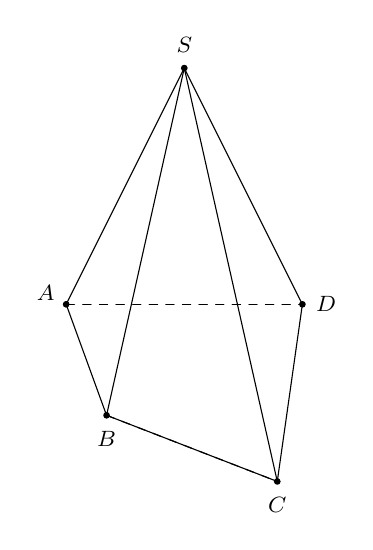
\begin{tikzpicture}[scale=1, font=\footnotesize, line join=round, line cap=round, >=stealth]
				\def \c{3.5} \def \b{1.5} \def \gb{-70} \def \gc{-40}
				\def \h{3} \def\d{3}
				\path
				(0,0) coordinate (A)
				(\gb:\b) coordinate (B)
				(\gc:\c) coordinate (C)
				(\d,0) coordinate (D)
				(\d/2,\h) coordinate (S)
				;
				\foreach \x/\y in {B/C,A/D}
				\draw[dashed] (\x)--(\y);
				\foreach \x/\y in {S/A,S/B,A/B,S/C,B/C,S/D,C/D}
				\draw[] (\x)--(\y);
				\foreach \x/\y in {A/150,B/-90,C/-90,D/0,S/90}
				\draw[fill] (\x) circle (1pt) +(\y:.3) node {$\x$};		
			\end{tikzpicture}
	}}
\end{ex}

\begin{ex}%[Dự án Toán 11-WTB-1]%[Lê Quốc Dũng]%[1K4B0-5]
	Cho hình chóp $S.ABCD$ có $ABCD$ là hình thang cân đáy lớn $AD$. Gọi $M$, $ N$ lần lượt là trung điểm của $AB$, $ CD$. Gọi $(P)$ là mặt phẳng qua $MN$ và cắt mặt bên $(SBC)$ theo một giao tuyến. Thiết diện của $(P)$ và hình chóp là 
	\choice
	{hình bình hành}
	{hình chữ nhật}
	{\True hình thang}
	{hình vuông}
	\loigiai{
		\immini{
			Giả sử mặt phẳng cắt theo giao tuyến $PQ$.\\
			Khi đó do $MN\parallel BC$ nên theo định lý ba giao tuyến song song hoặc đồng quy áp dụng cho ba mặt phẳng $(P)$; $(SBC)$; $(ABCD)$ thì ta được ba giao tuyến $MN$; $BC$; $PQ$ đôi một song song. \\Do đó thiết diện là một hình thang.}
		{\begin{tikzpicture}[scale=.7, font=\footnotesize, line join=round, line cap=round, >=stealth]
				\def \d{7} \def \l{-2} \def \c{2}
				\def \h{4}
				\path
				(0,0) coordinate (A)
				(\d,0) coordinate (D)
				(\d-\c,\l) coordinate (C)
				(\c,\l) coordinate (B)
				(\d/2,\h) coordinate (S)
				($(A)!.5!(B)$) coordinate (M)
				($(C)!.5!(D)$) coordinate (N)
				($(S)!.4!(B)$) coordinate (Q)
				($(S)!.4!(C)$) coordinate (P)
				;
				\foreach \x/\y in {D/C,A/D,M/N}
				\draw[dashed] (\x)--(\y);
				\foreach \x/\y in {S/A,S/D,A/B,S/C,D/C,S/B,C/B,P/Q,M/Q,N/P}
				\draw[] (\x)--(\y);
				\foreach \x/\y in {A/150,B/-90,C/-90,D/0,S/90,M/200,N/-30,P/30,Q/150}
				\draw[fill] (\x) circle (1pt) +(\y:.3) node {$\x$};		
			\end{tikzpicture}
	}}
\end{ex}
%---------------------------------------
\begin{ex}%[Dự án Toán 11-WTB-1]%[Lê Quốc Dũng]%[1K4B0-5]
	Cho tứ diện $ABCD$ đều cạnh $a$. Gọi $G$ là trọng tâm tam giác $ABC$, mặt phẳng $(CGD)$ cắt tứ diện theo một thiết diện có diện tích là 
	\choice
	{$\dfrac{a^2\sqrt{2}}{6}$}
	{$\dfrac{a^2\sqrt{3}}{4}$}
	{\True $\dfrac{a^2\sqrt{2}}{4}$}
	{$\dfrac{a^2\sqrt{3}}{2}$}
	\loigiai{
		\immini{
			Gọi giao điểm của $CG$ với $AB$ là $I$.\\ 
			Thiết diện của mặt phẳng $(CGD)$ với tứ diện $ABCD$ là tam giác $DCI$.\\
			Tam giác đều $ABC$ nên ta có $CI=\dfrac{a\sqrt{3}}{2}$.\\
			Tam giác đều $ABD$ nên ta có $DI=\dfrac{a\sqrt{3}}{2}$.\\
			Gọi $H$ là trung điểm của $CD$.\\
			Do $\triangle CDI$ có $CI=DI=\dfrac{a\sqrt{3}}{2}$ nên $IH \perp CD$ tại $H$.\\
			Áp dụg định lí Py-ta-go trong tam giác vuông $CIH$,\\ ta có $IH=\sqrt{CI^2-CH^2}=\sqrt{\dfrac{3a^2}{4}-\dfrac{a^2}{4}}=\dfrac{a\sqrt{2}}{2}$.\\
			Vậy $S_{DCI}=\dfrac{1}{2}\cdot IH\cdot CD =\dfrac{1}{2}\cdot \dfrac{a\sqrt{2}}{2} \cdot a=\dfrac{a^2\sqrt{2}}{4}.$}
		{\begin{tikzpicture}[scale=1, font=\footnotesize, line join=round, line cap=round, >=stealth]
				\def \c{4.5} \def \b{3} \def \gb{-60}
				\def \h{3}
				\path
				(0,0) coordinate (A)
				(\c,0) coordinate (C)
				(\gb:\c/2) coordinate (B)
				($(A)!.5!(B)$) coordinate (I)
				($(B)!.5!(C)$) coordinate (M)
				($(D)!.5!(C)$) coordinate (H)
				(intersection of A--M and C--I) coordinate (G)
				($(G)+(0,\h)$) coordinate (D)
				;
				\foreach \x/\y in {A/C,C/I,A/M,D/G,I/H}
				\draw[dashed] (\x)--(\y);
				\foreach \x/\y in {D/A,A/B,D/B,D/C,B/C,D/I}
				\draw (\x)--(\y);
				\foreach \x/\y in {A/150,B/-90,C/-90,D/90,I/180,G/-90,H/60}
				\draw[fill] (\x) circle (1pt) +(\y:.3) node {$\x$};		
			\end{tikzpicture}
	}}
\end{ex}

\begin{ex}%[Dự án Toán 11-WTB-1]%[Lê Quốc Dũng]%[1K4B0-5]
	Cho hình chóp $S.ABCD$ có đáy $ABCD$ là hình bình hành. Gọi $M$, $ N$, $ P$ lần lượt là trung điểm các cạnh $AB$, $ AD$, $ SC$. Thiết diện hình chóp với mặt phẳng $(MNP)$ là một
	\choice
	{tam giác}
	{tứ giác}
	{\True ngũ giác}
	{lục giác}
	\loigiai{
		\immini{
			Trong $(ABCD)$: $CD$ và $BC$ cắt $MN$ lần lượt tại $I$ và $E$.\\
			Trong $(SBC)$: $PI$ cắt $SB$ tại $J$. \\
			Trong $(SDC)$: $PE$ cắt $SD$ tại $K$.\\
			Khi đó $(MNP)$ giao với $(ABCD)$, $ (SDA)$, $ (SBC)$, $ (SAB)$, $ (SDC)$ lần lượt theo các giao tuyến $MN$, $NK$, $PJ$, $JM$, $KP$. \\
			Nên thiết diện tạo thành là ngũ giác $MNKPJ$.}
		{\begin{tikzpicture}[scale=1, font=\footnotesize, line join=round, line cap=round, >=stealth]
				\def \d{2} \def \b{4} \def \goc{45}
				\def \h{4}
				\path
				(0,0) coordinate (A)
				(\b,0) coordinate (B)
				(\goc:\d) coordinate (D)
				($(D)+(B)-(A)$) coordinate (C)	
				($(A)!.5!(C)$) coordinate (H)
				($(H)+(0,\h)$) coordinate (S)
				($(A)!.5!(B)$) coordinate (M)
				($(A)!.5!(D)$) coordinate (N)
				($(S)!.5!(C)$) coordinate (P)
				($(S)!.5!(D)$) coordinate (K)
				(intersection of M--N and B--C) coordinate (I)
				(intersection of M--N and D--C) coordinate (E)
				(intersection of S--B and P--I) coordinate (J)
				(intersection of S--D and P--E) coordinate (K)
				(intersection of S--A and P--E) coordinate (L)
				(intersection of S--A and I--E) coordinate (R)
				;
				\foreach \x/\y in {A/C,B/D,A/D,E/C,S/D,M/B,M/R,M/P,N/P,P/L,N/K}
				\draw[dashed] (\x)--(\y);
				\foreach \x/\y in {S/A,A/M,S/B,S/C,I/C,I/P,I/M,E/R,E/L, M/J}
				\draw[] (\x)--(\y);
				
				\foreach \x/\y in {A/150,B/-90,C/0,D/40,S/90,M/-90,N/-90,P/0,I/-90,E/180,J/10,K/-50}
				\draw[fill] (\x) circle (1pt) +(\y:.3) node {$\x$};		
			\end{tikzpicture}
	}}
\end{ex}

\begin{ex}%[Dự án Toán 11-WTB-1]%[Lê Quốc Dũng]%[1K4B0-5]
	Cho tứ diện $ABCD$. Trên các cạnh $AB$, $BC$, $CD$ lần lượt lấy các điểm $P$, $Q$, $R$ sao cho $AP=\dfrac{1}{3}AB$, $BQ=2QC$, $R$ không trùng với $C$, $D$. Gọi $PQRS$ là thiết diện của mặt phẳng $(PQR)$ với hình tứ diện $ABCD$. Khi đó $PQRS$ là
	\choice
	{hình thang cân}
	{\True hình thang}
	{một tứ giác không có cặp cạnh đối nào song song}
	{hình bình hành}
	\loigiai{
		\immini{
			Từ giả thiết, ta có $\dfrac{AP}{AB}=\dfrac{CQ}{CB}=\dfrac{1}{3}\Rightarrow PQ\parallel AC$.\\
			Giao tuyến của mặt phẳng $(PQR)$ và $(ACD)$ là đường thẳng đi qua $R$ và song song với $AC$, cắt $AD$ tại $S$.\\
			Do đó $PQRS$ là thiết diện của mặt phẳng $(PQR)$ với hình tứ diện $ABCD$.\\
			Theo cách dựng thì $PQ\parallel RS$ mà $R$ bất kỳ trên cạnh $CD$ nên thiết diện là hình thang.}
		{\begin{tikzpicture}[scale=1, font=\footnotesize, line join=round, line cap=round, >=stealth]
				\def \d{4} \def \c{2} \def \gb{-45}
				\def \h{3}
				\path
				(0,0) coordinate (B)
				(\d,0) coordinate (D)
				(\gb:\c) coordinate (C)
				($(B)!.5!(D)$) coordinate (H)
				($(H)+(0,\h)$) coordinate (A)
				($(A)!1/3!(B)$) coordinate (P)
				($(B)!2/3!(C)$) coordinate (Q)
				($(C)!.7!(D)$) coordinate (R)
				($(A)!.7!(D)$) coordinate (S)
				;
				\foreach \x/\y in {B/D,Q/R,P/S}
				\draw[dashed] (\x)--(\y);
				\foreach \x/\y in {A/B,A/C,A/D,B/C,C/D,P/Q,R/S}
				\draw[] (\x)--(\y);
				\foreach \x/\y in {A/150,B/180,C/-90,D/0,P/180,Q/180,R/-40,S/30}
				\draw[fill] (\x) circle (1pt) +(\y:.3) node {$\x$};		
			\end{tikzpicture}
	}}
\end{ex}

\begin{ex}%[Dự án Toán 11-WTB-1]%[Lê Quốc Dũng]%[1K4B0-5]
	Cho hình chóp $S.ABCD$. Có đáy $ABCD$ là hình bình hành. Gọi $M$, $N$, $Q$ lần lượt là trung điểm của các cạnh $AB$, $AD$, $SC$. Thiết diện của hình chóp với mặt phẳng $(MNQ)$ là đa giác có bao nhiêu cạnh?
	\choice
	{$3$}
	{$4$}
	{\True $5$}
	{$6$}
	\loigiai{
		\immini{
			Trong $(ABCD)$, gọi $K=MN\cap CD$, $L=MN\cap BC$ suy ra $K\in (SCD)$, $L\in (SBC)$.\\
			Trong $(SCD)$, gọi $P=KQ\cap SD$.\\
			Trong $(SBC)$, gọi $R=LQ\cap SB$.\\
			Khi đó ta có: $(MNQ)\cap (ABCD)=MN$; $(MNQ)\cap (SAD)=NP$; $(MNQ)\cap (SCD)=PQ$; $(MNQ)\cap (SBC)=QR$; $(MNQ)\cap (SAB)=RM$.\\
			Vậy thiết diện cần tìm là ngũ giác.}
		{\begin{tikzpicture}[scale=.7, font=\footnotesize, line join=round, line cap=round, >=stealth]
				\def \b{4} \def \d{2.5} \def \goc{-145}
				\def \h{3}
				\path
				(0,0) coordinate (A)
				(\b,0) coordinate (B)
				(\goc:\d) coordinate (D)
				($(B)+(D)-(A)$) coordinate (C)	
				(0,\h) coordinate (S)
				($(A)!.5!(B)$) coordinate (M)
				($(A)!.5!(D)$) coordinate (N)
				($(S)!.5!(C)$) coordinate (Q)
				(intersection of M--N and C--D) coordinate (K)
				(intersection of M--N and B--C) coordinate (L)
				(intersection of K--Q and S--D) coordinate (P)
				(intersection of L--Q and S--B) coordinate (R)
				;
				\fill[cyan] (M)--(N)--(P)--(Q)--(R)--cycle;
				\foreach \x/\y in {S/A,A/D,A/B,K/L,N/P,M/R}
				\draw[dashed] (\x)--(\y);
				\foreach \x/\y in {S/D,S/C,S/B,K/C,C/L,K/Q,Q/L}
				\draw[] (\x)--(\y);
				
				\foreach \x/\y in {A/40,B/0,C/-90,D/-90,S/90,M/-90,N/-30,Q/30,K/180,L/0,R/90,P/150}
				\draw[fill] (\x) circle (1pt) +(\y:.3) node {$\x$};		
			\end{tikzpicture}
	}}
\end{ex}

\begin{ex}%[Dự án Toán 11-WTB-1]%[Lê Quốc Dũng]%[1K4B0-5]
	\immini{Cho hình chóp $S.ABCD$ có đáy là hình thang, $AB\parallel CD$ và $AB=2CD$. Gọi $O$ là giao điểm của $AC$ và $BD$. Lấy $E$ thuộc cạnh $SA$, $F$ thuộc cạnh $SC$ sao cho $\dfrac{SE}{SA}=\dfrac{SF}{SC}=\dfrac{2}{3}$. Thiết diện của hình chóp $S.ABCD$ cắt bởi mặt phẳng $(BEF)$ là
		\choice
		{một tam giác}
		{\True một tứ giác}
		{một hình thang}
		{một hình bình hành}}
	{\begin{tikzpicture}[scale=.7, font=\footnotesize, line join=round, line cap=round, >=stealth]
			\def \b{8} \def \l{-2} 
			\pgfmathsetmacro \c{\b/4}
			\def \h{5}
			\path
			(0,0) coordinate (A)
			(\b,0) coordinate (B)
			(\b-\c,\l) coordinate (C)
			(\c,\l) coordinate (D)
			(\b/2,\h) coordinate (S)
			(intersection of A--C and B--D) coordinate (O)
			($(S)!2/3!(A)$) coordinate (E)
			($(S)!2/3!(C)$) coordinate (F)
			;
			\foreach \x/\y in {B/C,A/B,A/C,B/D,E/B,E/F}
			\draw[dashed] (\x)--(\y);
			\foreach \x/\y in {S/A,S/B,A/D,S/C,B/C,S/D,C/D,B/F}
			\draw[] (\x)--(\y);
			\foreach \x/\y in {A/150,B/0,C/-90,D/-90,S/90,O/-90,E/180,F/-150}
			\draw[fill] (\x) circle (1pt) +(\y:.25) node {$\x$};		
		\end{tikzpicture}
	}
	\loigiai{
		\immini{
			Trong $(SAC)$, gọi $I=SO\cap EF$, trong $(SBD)$, gọi $N=BI\cap SD$.\\
			Suy ra $N$ là giao điểm của đường thẳng $SD$ với mặt phẳng $(BEF)$.\\
			Thiết diện của hình chóp cắt bởi mặt phẳng $(BEF)$ là tứ giác $BFNE$.}
		{\begin{tikzpicture}[scale=.7, font=\footnotesize, line join=round, line cap=round, >=stealth]
				\def \b{8} \def \l{-2} 
				\pgfmathsetmacro \c{\b/4}
				\def \h{5}
				\path
				(0,0) coordinate (A)
				(\b,0) coordinate (B)
				(\b-\c,\l) coordinate (C)
				(\c,\l) coordinate (D)
				(\b/2,\h) coordinate (S)
				(intersection of A--C and B--D) coordinate (O)
				($(S)!2/3!(A)$) coordinate (E)
				($(S)!2/3!(C)$) coordinate (F)
				(intersection of S--O and E--F) coordinate (I)
				(intersection of S--D and B--I) coordinate (N)
				;
				\foreach \x/\y in {B/C,A/B,A/C,B/D,E/B,E/F,S/O,N/B}
				\draw[dashed] (\x)--(\y);
				\foreach \x/\y in {S/A,S/B,A/D,S/C,B/C,S/D,C/D,B/F,E/N,N/F}
				\draw[] (\x)--(\y);
				\foreach \x/\y in {A/150,B/0,C/-90,D/-90,S/90,O/-90,E/180,F/-150,I/-135,N/220}
				\draw[fill] (\x) circle (1pt) +(\y:.3) node {$\x$};		
			\end{tikzpicture}
	}}
\end{ex}

\begin{ex}%[Dự án Toán 11-WTB-1]%[Lê Quốc Dũng]%[1K4B0-5]
	Cho hình chóp $S.ABCD$ có đáy $ABCD$ là hình thang với đáy lớn $AD$, $E$ là trung điểm của cạnh $SA$, $F$, $G$ là các điểm thuộc cạnh $SC$, $AB$ ($F$ không là trung điểm của $SC)$. Thiết diện của hình chóp cắt bởi mặt phẳng $(EFG)$ là một hình
	\choice
	{lục giác}
	{\True ngũ giác}
	{tam giác}
	{tứ giác}
	\loigiai{
		\immini{
			Gọi $N=EG\cap SB$; $K=NF\cap BC$; $O=AC\cap BD$; $I=FE\cap SO$; $H=NI\cap SD$.\\
			Khi đó, ta có  $(SAB)\cap (EGF)=EG$; $(ABCD)\cap (EGF)=GK$;\\
			$(EGF)\cap (SBC)=KF$; $(EGF)\cap (SCD)=FH$; $(EGF)\cap (SAD)=EH.$
			Vậy thiết diện của hình chóp cắt bởi mặt phẳng $(EGF)$ là ngũ giác $EGKFH$.}
		{\begin{tikzpicture}[scale=1, font=\footnotesize, line join=round, line cap=round, >=stealth]
				\def \b{2} \def \d{7} \def \l{-2} 
				\def \h{5}
				\path
				(0,0) coordinate (A)
				(\d,0) coordinate (D)
				(\b,\l) coordinate (B)
				($(B)+(2,0)$) coordinate (C)
				(\b/2,\h) coordinate (S)
				($(S)!.5!(A)$) coordinate (E)
				($(S)!2/3!(C)$) coordinate (F)
				($(A)!.8!(B)$) coordinate (G)
				(intersection of E--G and S--B) coordinate (N)
				(intersection of N--F and B--C) coordinate (K)
				(intersection of A--C and B--D) coordinate (O)
				(intersection of E--F and S--O) coordinate (I)
				(intersection of N--I and S--D) coordinate (H)
				;
				\fill[gray!20] (E)--(H)--(F)--(K)--(G)--cycle;
				\foreach \x/\y in {A/D,G/F,F/E,A/C,B/D,S/O,N/H,E/H,G/K}
				\draw[dashed] (\x)--(\y);
				\foreach \x/\y in {S/A,S/N,S/C,S/D,A/B,B/C,C/D,E/N,N/F,F/H}
				\draw (\x)--(\y);
				\foreach \x/\y in {A/150,C/-90,D/0,S/90,E/180,F/0,G/-160,N/0,K/-45,O/60,I/-150,H/60}
				\draw[fill] (\x) circle (1pt) +(\y:.3) node {$\x$};	
				\foreach \x/\y in {B/-145}
				\draw[fill] (\x) circle (1pt) +(\y:.2) node {$\x$};		
		\end{tikzpicture}}
	}
\end{ex}

\begin{ex}%[Dự án Toán 11-WTB-1]%[Cao Thành Thái]%[1K4KA-5]
Cho hình chóp $S.ABCD$ có đáy $ABCD$ là hình bình hành. Gọi $I$ là trung điểm của $SA$. Thiết diện của hình chóp $S.ABCD$ cắt bởi $(IBC)$ là
\choice
{tứ giác $IBCD$}
{hình thang $IGBC$ ($G$ là trung điểm của $SB$)}
{\True hình thang $IJCB$ ($J$ là trung điểm của $SD$)}
{tam giác $IBC$}
\loigiai
{
\immini
{
Gọi $J$ là trung điểm của $SD$. Khi đó $IJ$ là đường trung bình của tam giác $SAD$, suy ra $IJ\parallel AD$. Mà $AD\parallel BC$ nên $IJ\parallel BC$, thêm nữa $I\in (IBC)$. Do đó, $J\in (IBC)$.\\
Ta có $\left\{\begin{aligned}&(IBC)\cap (ABCD)=BC \\&(IBC)\cap (SBC)=BC \\&(IBC)\cap (SAB)=IB\\&(IBC)\cap (SAD)=IJ \\&(IBC)\cap (SCD)=JC.\end{aligned}\right.$\\
Vậy thiết diện của hình chóp $S.ABCD$ cắt bởi $(IBC)$ là hình thang $IJCB$ (do $IJ\parallel BC$).
}
{
\begin{tikzpicture}[line cap=round,line join=round,font=\footnotesize,scale=.8]
	\path (0:0) coordinate(A) (0:3) coordinate(B) (-135:1.4) coordinate(D) ($(B)+(D)-(A)$) coordinate(C) (100:2.6) coordinate(S) ($(S)!.5!(A)$) coordinate(I) ($(S)!.5!(D)$) coordinate(J);
	\draw (S)--(B)--(C)--(D)--cycle (S)--(C)--(J);
	\draw[dashed] (S)--(A)--(B) (A)--(D) (B)--(I)--(J);
	\foreach \d/\g in {A/170, B/0, C/-45, D/-135, S/90, I/60, J/180}
	\fill (\d) circle(1pt) node[shift={(\g:.3)}]{$\d$};
\end{tikzpicture}
}
}
\end{ex}

\begin{ex}%[Dự án Toán 11-WTB-1]%[Cao Thành Thái]%[1K4K0-5]
\immini
{
Cho tứ diện đều $ABCD$ có cạnh bằng $2$. Gọi $G$ là trọng tâm tam giác $ABC$. Cắt tứ diện bởi mặt phẳng $(GCD)$ ta được thiết diện có diện tích bằng
\choice
{$\sqrt{3}$}
{$2\sqrt{3}$}
{\True $\sqrt{2}$}
{$\dfrac{2\sqrt{2}}{3}$}
}
{
\begin{tikzpicture}[line cap=round,line join=round,font=\footnotesize,scale=.6]
	\def\a{2}
	\pgfmathsetmacro\b{\a*cos(30)}
	\path (180:\a)  coordinate (A) (0:\a)coordinate (C) (-120:\b) coordinate (B) ($(B)!.5!(C)$) coordinate (N) ($(A)!.5!(B)$) coordinate (M) (intersection of A--N and C--M) coordinate (G) ++(90:1.5*\a) coordinate (D);
	\draw[dashed] (A)--(C) (A)--(N) (C)--(M) (D)--(G);
	\draw (A)--(B)--(C)--(D)--cycle (D)--(B);
	\foreach \d/\g in {A/180, B/-100, C/0, D/90, G/-100} \fill (\d) circle (1pt) node[shift={(\g:.3)}]{$\d$};
\end{tikzpicture}
}
\loigiai
{
\immini
{
Gọi $M$ là trung điểm của $AB$. Khi đó $M\in CG$, suy ra $M\in (GCD)$.\\
Ta có $\left\{\begin{aligned}&(GCD)\cap (ABC)=CM \\&(GCD)\cap (ABD)=DM \\&(GCD)\cap (ACD)=CD \\&(GCD)\cap (BCD)=CD.\end{aligned}\right.$\\
Vậy thiết diện của tứ diện $ABCD$ cắt bởi $(GCD)$ là tam giác $CDM$.\\
Tam giác $ABC$ đều cạnh bằng $2$ nên $CM=\dfrac{2\sqrt{3}}{2}=\sqrt{3}$.\\
Tam giác $ABD$ đều cạnh bằng $2$ nên $DM=\dfrac{2\sqrt{3}}{2}=\sqrt{3}$.
}
{
\begin{tikzpicture}[line cap=round,line join=round,font=\footnotesize,scale=1]
	\def\a{2}
	\pgfmathsetmacro\b{\a*cos(30)}
	\path (180:\a)  coordinate (A) (0:\a)coordinate (C) (-120:\b) coordinate (B) ($(B)!.5!(C)$) coordinate (N) ($(A)!.5!(B)$) coordinate (M) (intersection of A--N and C--M) coordinate (G) ++(90:1.5*\a) coordinate (D);
	\draw[dashed] (A)--(C) (A)--(N) (C)--(M) (D)--(G);
	\draw (A)--(B)--(C)--(D)--cycle (D)--(B) (D)--(M);
	\foreach \d/\g in {A/180, B/-100, C/0, D/90, G/-100, M/-140} \fill (\d) circle (1pt) node[shift={(\g:.3)}]{$\d$};
\end{tikzpicture}
}
\noindent
Nửa chu vi của tam giác $CDM$ là $p=\dfrac{CD+CM+DM}{2} = \dfrac{2+\sqrt{3}+\sqrt{3}}{2}=\sqrt{3}+1$.\\
Diện tích của tam giác $CDM$ là $S=\sqrt{p(p-CD)(p-CM)(p-DM)} = \sqrt{2}$.
}
\end{ex}

\begin{ex}%[Dự án Toán 11-WTB-1]%[Cao Thành Thái]%[1K4G0-5]
Cho khối lập phương $ABCD.A'B'C'D'$ cạnh $a$. Các điểm $E$, $F$ lần lượt là trung điểm của $C'B'$ và $C'D'$. Diện tích thiết diện của khối lập phương cắt bởi mặt phẳng $(AEF)$ bằng
\choice
{\True $\dfrac{7a^2\sqrt{17}}{24}$}
{$\dfrac{a^2\sqrt{17}}{4}$}
{$\dfrac{a^2\sqrt{17}}{8}$}
{$\dfrac{7a^2\sqrt{17}}{12}$}
\loigiai
{
\immini
{
Vì $EF$ là đường trung bình của tam giác $B'C'D'$ nên $EF\parallel B'D'$. Mà $B'D'\parallel BD$ nên $EF\parallel BD$.\\
Trong mặt phẳng $(ABCD)$, qua $A$ dựng đường thẳng song song với $BD$, cắt $CD$, $CB$ lần lượt tại $I$ và $J$. Khi đó, $I\in \left(CDD'C'\right)$ và $J\in \left(BCC'B'\right)$.\\
Trong mặt phẳng $\left(CDD'C'\right)$, gọi $G$ là giao điểm của $IF$ và $DD'$.\\
Trong mặt phẳng $\left(BCC'B'\right)$, gọi $K$ là giao điểm của $JE$ và $BB'$.\\
Khi đó, ta có $\left\{\begin{aligned}&(AEF)\cap \left(A'B'C'D'\right)=EF \\&(AEF)\cap \left(CDD'C'\right)=FG \\&(AEF)\cap \left(ADD'A'\right)=AG \\&(AEF)\cap \left(ABB'A'\right)=AK \\&(AEF)\cap \left(BCC'B'\right)=KE.\end{aligned}\right.$\\
Vậy thiết diện của khối lập phương $ABCD.A'B'C'D'$ cắt bởi mặt phẳng $(AEF)$ là ngũ giác $AKEFG$.
}
{
\begin{tikzpicture}[line cap=round,line join=round,font=\footnotesize,scale=1]
\def\a{3.5}
\path (0:0) coordinate (A) (0:\a) coordinate (B) ++(40:\a/2) coordinate (C) +(180:\a) coordinate (D)
\foreach \d in {A,B,C,D}{(\d)++(90:\a) coordinate (\d')};
\path ($(B')!.5!(C')$) coordinate(E) ($(D')!.5!(C')$) coordinate(F) ($(A)+(F)-(E)$) coordinate(i) (intersection of A--i and C--D) coordinate (I) (intersection of A--i and C--B) coordinate (J) (intersection of E--J and B--B') coordinate (K) (intersection of F--I and D--D') coordinate (G) (intersection of F--I and A--A') coordinate (j) (intersection of J--E and C--C') coordinate (H);
\draw[dashed] (D')--(D)--(A) (C)--(D) (E)--(A)--(F)--(j) (A)--(G)--(K) (I)--(D) (F)--(C') (A)--(B)--(D);
\draw (A')--(A) (B)--(C)--(H) (B)--(B') (A')--(B')--(C') (A')--(D')--(F)--(E)--(J)--(I)--(j) (J)--(B) (B')--(D') (F)--(H)--(E) (A)--(K);
\foreach \d/\g in {A/-135, B/-30, C/0, A'/180, B'/90, C'/45, D'/135, E/-20, F/90, I/180, J/-90, K/-20, H/45}
\fill (\d) circle(1pt) node[shift={(\g:.3)}]{$\d$};
\fill (D) circle(1pt) node[shift={(35:.35)}]{$D$} (G) circle(1pt) node[shift={(140:.35)}]{$G$};
\end{tikzpicture}
}
\noindent
Gọi $H$ là giao điểm của $IF$ và $JE$.\\
Vì $\left\{\begin{aligned}&(IJEF)\cap \left(BCC'B'\right)=JE \\&(IJEF)\cap \left(CDD'C'\right)=IF \\&\left(BCC'B'\right)\cap \left(CDD'C'\right)=CC' \\&IF\cap JE=H\end{aligned}\right.$ nên các đường thẳng $IF$, $JE$, $CC'$ đồng quy tại $H$, tức là $H\in CC'$.\\
Tứ giác $ADBJ$ có $AD\parallel BJ$ và $BD\parallel AJ$ nên $ADBJ$ là hình bình hành. Suy ra $BJ=AD=BC=a$.\\
Ta có $\dfrac{B'K}{BK}=\dfrac{B'E}{BJ} = \dfrac{B'E}{BC}=\dfrac{1}{2}$. Suy ra $B'K=\dfrac{1}{3}BB'=\dfrac{a}{3}$ và $BK=\dfrac{2a}{3}$.\\
Xét hai tam giác vuông $EKB'$ và $EHC'$ có $\widehat{EB'K}=\widehat{EC'H}=90^\circ$, $B'E=C'E$, $\widehat{B'EK}=\widehat{C'EH}$ (hai góc đối đỉnh).\\
Do đó, $\triangle EKB' = \triangle EHC'$. Suy ra $C'H=B'K=\dfrac{a}{3}$ và $EH=EK$.\\
Tương tự, ta cũng có $FH=FG$.\\
Ta có $KH=2EK=2\sqrt{B'E^2+B'K^2} = 2\sqrt{\dfrac{a^2}{4}+\dfrac{a^2}{9}} = \dfrac{a\sqrt{13}}{3}$.\\
Lại có $AK=\sqrt{AB^2+BK^2} = \sqrt{a^2+\dfrac{4a^2}{9}} = \dfrac{a\sqrt{13}}{3}$.\\
Suy ra $AK=KH$.\\
Chứng minh tương tự, ta cũng có $AG=GH$.\\
Do đó, $AGHK$ là hình thoi.\\
Vì $EF$ là đường trung bình của tam giác $GHK$ nên $GK=2EF=B'D'=a\sqrt{2}$.\\
Trong tam giác $ACH$ vuông tại $C$ ta có $AH=\sqrt{AC^2+CH^2} = \sqrt{2a^2+\left(a+\dfrac{a}{3}\right)^2} = \dfrac{a\sqrt{34}}{3}$.\\
Diện tích hình thoi $AGHK$ là $S_{AGHK}=\dfrac{1}{2}GK\cdot AH = \dfrac{1}{2}\cdot a\sqrt{2}\cdot \dfrac{a\sqrt{34}}{3} = \dfrac{a^2\sqrt{17}}{3}$.\\
Diện tích tam giác $EFH$ là $S_{EFH}=\dfrac{1}{4}S_{GHK}=\dfrac{1}{8}S_{AGHK} = \dfrac{a^2\sqrt{17}}{24}$.\\
Diện tích ngũ giác $AKEFG$ là $S_{AKEFG}=S_{AGHK}-S_{GHK} = \dfrac{a^2\sqrt{17}}{3}-\dfrac{a^2\sqrt{17}}{24} = \dfrac{7a^2\sqrt{17}}{24}$.
}
\end{ex}

\begin{ex}%[Dự án Toán 11-WTB-1]%[Cao Thành Thái]%[1K4K0-5]
Cho hình chóp $S.ABCD$. Gọi $M$, $N$ lần lượt là trung điểm của $SB$ và $SD$. Thiết diện của hình chóp $S.ABCD$ và mặt phẳng $(AMN)$ là hình gì?
\choice
{Tam giác vuông}
{Ngũ giác}
{Tam giác cân}
{\True Tứ giác}
\loigiai
{
\immini
{
Gọi $O$ là giao điểm của $AC$ và $BD$. Suy ra $SO$ là giao tuyến của hai mặt phẳng $(SAC)$ và $(SBD)$.\\
Trong mặt phẳng $(SBD)$, gọi $I$ là giao điểm của $SO$ và $MN$.\\
Trong mặt phẳng $(SAC)$, gọi $P$ là giao điểm của $AI$ và $SC$. Suy ra $P\in (AMN)$.\\
Khi đó, ta có $\left\{\begin{aligned}&(AMN)\cap (SAB)=AM \\&(AMN)\cap (SBC)=MP \\&(AMN)\cap (SCD)=PN \\&(AMN)\cap (SAD)=AN.\end{aligned}\right.$\\
Vậy thiết diện của hình chóp $S.ABCD$ và mặt phẳng $(AMN)$ là tứ giác $AMPN$.
}
{
\begin{tikzpicture}[line cap=round,line join=round,font=\footnotesize,scale=1]
	\path (0:0) coordinate(A) (0:3.5) coordinate(B) ++(-130:1.8) coordinate(C) (-75:1) coordinate(D) (70:3) coordinate(S) ($(S)!.5!(B)$) coordinate(M) ($(S)!.5!(D)$) coordinate(N) (intersection of A--C and B--D) coordinate (O) (intersection of S--O and M--N) coordinate (I) (intersection of A--I and S--C) coordinate (P);
	\draw (S)--(B)--(C)--(D)--(A)--cycle (S)--(C) (S)--(D) (A)--(N)--(P)--(M);
	\draw[dashed] (A)--(B) (A)--(M)--(N) (A)--(C) (B)--(D) (S)--(O) (A)--(P);
	\foreach \d/\g in {A/180, B/0, C/-45, D/-135, S/90, M/20, O/-95, P/40}
	\fill (\d) circle(1pt) node[shift={(\g:.25)}]{$\d$};
	\fill (N) circle(1pt) node[shift={(180:.16)}]{$N$} (I) circle(1pt) node[shift={(-45:.2)}]{$I$};
\end{tikzpicture}
}
}
\end{ex}

\begin{ex}%[Dự án Toán 11-WTB-1]%[Cao Thành Thái]%[1K4K0-5]
Cho hình chóp $S.ABCD$ có đáy $ABCD$ là hình bình hành. Gọi $M$, $N$, $K$ lần lượt là trung điểm của $CD$, $CB$, $SA$. Thiết diện của hình chóp cắt bởi mặt phẳng $(MNK)$ là một đa giác $(\mathcal{H})$. Khẳng định nào dưới đây đúng?
\choice
{$(\mathcal{H})$ là một hình thang có hai đáy không bằng nhau}
{$(\mathcal{H})$ là hình bình hành}
{\True $(\mathcal{H})$ là một ngũ giác}
{$(\mathcal{H})$ là một tam giác}
\loigiai
{
\immini
{
Trong mặt phẳng $(ABCD)$, gọi $E$, $F$ lần lượt là giao điểm của $MN$ với $AB$, $AD$. Suy ra $E\in (SAB)$, $F\in (SAD)$.\\
Trong mặt phẳng $(SAB)$, gọi $G$ là giao điểm của $EK$ và $SB$. Suy ra $G\in (MNK)$.\\
Trong mặt phẳng $(SAD)$, gọi $H$ là giao điểm của $FK$ và $SD$. Suy ra $H\in (MNK)$.\\
Khi đó, ta có $\left\{\begin{aligned}&(MNK)\cap (ABCD)=MN \\&(MNK)\cap (SBC)=NG \\&(MNK)\cap (SAB)=GK \\&(MNK)\cap (SAD)=KH \\&(MNK)\cap (SCD)=HM.\end{aligned}\right.$
}
{
\begin{tikzpicture}[line cap=round,line join=round,font=\footnotesize,scale=1]
	\path (0:0) coordinate(A) (-135:1.5) coordinate(B) ++(0:3) coordinate(C) ($(A)+(C)-(B)$) coordinate(D) (100:3.2) coordinate(S) ($(C)!.5!(D)$) coordinate(M) ($(C)!.5!(B)$) coordinate(N) ($(S)!.5!(A)$) coordinate(K);
	\path (intersection of M--N and A--B) coordinate (E) (intersection of M--N and A--D) coordinate (F) (intersection of K--E and S--B) coordinate (G) (intersection of K--F and S--D) coordinate (H);
	\draw (S)--(C)--(N) (C)--(M) (N)--(E)--(G)--cycle (M)--(H)--(F)--cycle (S)--(G) (S)--(H);
	\draw[dashed] (S)--(A)--(B) (A)--(D) (M)--(N)--(K)--cycle (G)--(K)--(H) (G)--(B)--(N) (B)--(E) (M)--(D)--(H) (D)--(F);
	\foreach \d/\g in {A/180, B/-45, C/-45, D/45, S/90, M/-45, N/-85, K/40, E/-135, F/0, G/180, H/45}
	\fill (\d) circle(1pt) node[shift={(\g:.25)}]{$\d$};
\end{tikzpicture}
}
\noindent
Vậy thiết diện của hình chóp $S.ABCD$ cắt bởi mặt phẳng $(MNK)$ là ngũ giác $MNGKH$.
}
\end{ex}

\begin{ex}%[Dự án Toán 11-WTB-1]%[Cao Thành Thái]%[1K4K0-5]
Cho hình chóp tứ giác $S.ABCD$. Gọi $C'$ là điểm trên cạnh $SC$ sao cho $SC'=\dfrac{2}{3}SC$. Thiết diện của hình chóp với mặt phẳng $\left(ABC'\right)$ là một đa giác $m$ cạnh. Giá trị của $m$ là
\choice
{$m=6$}
{\True $m=4$}
{$m=5$}
{$m=3$}
\loigiai
{
\immini
{
Gọi $O$ là giao điểm của $AC$ và $BD$. Suy ra $SO$ là giao tuyến của hai mặt phẳng $(SAC)$ và $(SBD)$.\\
Trong mặt phẳng $(SAC)$, gọi $I$ là giao điểm của $SO$ và $AC'$.\\
Trong mặt phẳng $(SBD)$, gọi $E$ là giao điểm của $BI$ và $SD$. Suy ra $E\in \left(ABC'\right)$.\\
Khi đó, ta có $\left\{\begin{aligned}&\left(ABC'\right)\cap (ABCD)=AB \\&\left(ABC'\right)\cap (SAB)=AB \\&\left(ABC'\right)\cap (SBC)=BC' \\&\left(ABC'\right)\cap (SCD)=C'E \\&\left(ABC'\right)\cap (SAD)=EA.\end{aligned}\right.$
}
{
\begin{tikzpicture}[line cap=round,line join=round,font=\footnotesize,scale=1]
	\path (0:0) coordinate(A) (0:3.5) coordinate(D) ++(-130:2) coordinate(C) (-75:1) coordinate(B) (70:3) coordinate(S) ($(S)!{2/3}!(C)$) coordinate(C') (intersection of A--C and B--D) coordinate (O) (intersection of S--O and A--C') coordinate (I) (intersection of B--I and S--D) coordinate (E);
	\draw (S)--(A)--(B)--(C)--(D)--cycle (S)--(C) (S)--(B) (E)--(C')--(B);
	\draw[dashed] (A)--(D) (A)--(C) (A)--(C') (A)--(E) (B)--(D) (S)--(O) (B)--(E);
	\foreach \d/\g in {A/180, B/-135, C/-45, D/0, S/90, O/-95, E/40, C'/-20}
	\fill (\d) circle(1pt) node[shift={(\g:.25)}]{$\d$};
	\fill (I) circle(1pt) node[shift={(-45:.2)}]{$I$};
\end{tikzpicture}
}
\noindent
Do đó, thiết diện của hình chóp $S.ABCD$ với mặt phẳng $\left(ABC'\right)$ là tứ giác $ABC'E$.\\
Vậy $m=4$.
}
\end{ex}

\begin{ex}%[Dự án Toán 11-WTB-1]%[Cao Thành Thái]%[1K4K0-5]
Cho tứ diện $ABCD$ có $M$, $N$ lần lượt là trung điểm của $AB$, $CD$ và $P$ là một điểm thuộc cạnh $BC$ ($P$ không là trung điểm của $BC$). Thiết diện của tứ diện bị cắt bởi mặt phẳng $(MNP)$ là
\choice
{\True tứ giác}
{ngũ giác}
{lục giác}
{tam giác}
\loigiai
{
\immini
{
Vì $P$ không là trung điểm của $BC$ nên $MP$ không song song với $AC$.\\
Trong mặt phẳng $(ABC)$, gọi $E$ là giao điểm của $MP$ và $AC$. Suy ra $E$ thuộc cả hai mặt phẳng $(MNP)$ và $(ACD)$.\\
Trong mặt phẳng $(ACD)$, gọi $Q$ là giao điểm của $EN$ và $AD$. Suy ra $Q\in (MNP)$.\\
Khi đó, ta có $\left\{\begin{aligned}&(MNP)\cap (ABC)=MP \\&(MNP)\cap (BCD)=PN \\&(MNP)\cap (ACD)=NQ \\&(MNP)\cap (ABD)=QM.\end{aligned}\right.$\\
Vậy thiết diện của tứ diện $ABCD$ cắt bởi mặt phẳng $(MNP)$ là tứ giác $MPNQ$.
}
{
\begin{tikzpicture}[line cap=round,line join=round,font=\footnotesize,scale=1]
	\path (0:0) coordinate(B) (-40:2.5) coordinate(C) (0:4) coordinate(D) (55:3.2) coordinate(A) ($(A)!.5!(B)$) coordinate(M) ($(C)!.5!(D)$) coordinate(N) ($(B)!.7!(C)$) coordinate(P);
	\path (intersection of M--P and A--C) coordinate (E) (intersection of E--N and A--D) coordinate (Q);
	\draw (A)--(B)--(C)--(D)--cycle (A)--(E) (M)--(E)--(Q);
	\draw[dashed] (B)--(D) (M)--(Q) (N)--(P);
	\foreach \d/\g in {A/90, B/180, C/-45, D/0, M/135, N/-35, P/-150, E/-90, Q/45}
	\fill (\d) circle(1pt) node[shift={(\g:.25)}]{$\d$};
\end{tikzpicture}
}
}
\end{ex}

\begin{ex}%[Dự án Toán 11-WTB-1]%[Cao Thành Thái]%[1K7KM-5]
Cho hình lập phương $ABCD.A'B'C'D'$ có cạnh bằng $a$ ($a>0$). Thiết diện của hình lập phương đã cho cắt bởi mặt phẳng trung trực của đoạn $AC'$ có diện tích bằng
\choice
{$\dfrac{2\sqrt{2}}{3}a^2$}
{$a^2$}
{\True $\dfrac{3\sqrt{3}}{4}a^2$}
{$\dfrac{\sqrt{5}}{2}a^2$}
\loigiai
{
\immini
{
Gọi $E$, $F$, $G$, $H$, $I$, $J$ lần lượt là trung điểm của $BC$, $CD$, $DD'$, $A'D'$, $A'B'$, $BB'$.\\
Ta có $C'E=\sqrt{C'C^2+EC^2} = \sqrt{a^2+\dfrac{a^2}{4}} = \dfrac{a\sqrt{5}}{2}$.\\
Lại có $AE=\sqrt{AB^2+BE^2} = \sqrt{a^2+\dfrac{a^2}{4}} = \dfrac{a\sqrt{5}}{2}$.\\
Suy ra $AE=C'E$ hay $E$ thuộc mặt phẳng trung trực của đoạn thẳng $AC'$.\\
Chứng minh tương tự, ta cũng có $F$, $G$, $H$, $I$, $J$ thuộc mặt phẳng trung trực của đoạn thẳng $AC'$.\\
Vì $EF$ là đường trung bình của tam giác $BCD$ nên $EF=\dfrac{BD}{2}=\dfrac{a\sqrt{2}}{2}$.\\
Tương tự, $FG=GH=HI=IJ=JE=\dfrac{a\sqrt{2}}{2}$.
}
{
\begin{tikzpicture}[line cap=round,line join=round,font=\footnotesize,scale=1]
	\def\a{3.5}
	\path (0:0) coordinate (A) (0:\a) coordinate (B) ++(45:\a/2) coordinate (C) +(180:\a) coordinate (D)
	\foreach \d in {A,B,C,D}{(\d)++(-90:\a) coordinate (\d')};
	\path ($(B)!.5!(C)$) coordinate(E) ($(C)!.5!(D)$) coordinate(F) ($(D')!.5!(D)$) coordinate(G) ($(A')!.5!(D')$) coordinate(H) ($(A')!.5!(B')$) coordinate(I) ($(B)!.5!(B')$) coordinate(J);
	\draw[dashed] (D)--(D')--(A') (C')--(D') (A)--(C') (F)--(G)--(H)--(I);
	\draw (A)--(A')--(B')--(C')--(C) (B)--(B') (A)--(B)--(C)--(D)--cycle (F)--(E)--(J)--(I) (B)--(D);
	\foreach \d/\g in {A/180, B/-20, C/45, D/135, A'/-135, B'/-45, C'/0, D'/180, E/-20, F/90, G/-10, H/180, I/-90, J/-45}
	\fill (\d) circle(1pt) node[shift={(\g:.3)}]{$\d$};
\end{tikzpicture}
}
\noindent
Vậy thiết diện của hình lập phương đã cho cắt bởi mặt phẳng trung trực của đoạn $AC'$ là lục giác đều $EFGHIJ$ có cạnh bằng $\dfrac{a\sqrt{2}}{2}$.\\
Diện tích lục giác đều $EFGHIJ$ là $S=6\cdot \left(\dfrac{a\sqrt{2}}{2}\right)^2\cdot \dfrac{\sqrt{3}}{4} = \dfrac{3a^2\sqrt{3}}{4}$.
}
\end{ex}

\begin{ex}%[Dự án Toán 11-WTB-1]%[Cao Thành Thái]%[1K4K0-5]
Cho hình chóp $S.ABCD$, $G$ là điểm nằm trong tam giác $SCD$. $E$, $F$ lần lượt là trung điểm của $AB$ và $AD$. Thiết diện của hình chóp khi cắt bởi mặt phẳng $(EFG)$ là
\choice
{tam giác}
{tứ giác}
{\True ngũ giác}
{lục giác}
\loigiai
{
\immini
{
Trong mặt phẳng $(ABCD)$, gọi $H$, $I$ lần lượt là giao điểm của $EF$ với $BC$, $CD$. Suy ra $H\in (SBC)$, $I\in (SCD)$.\\
Trong mặt phẳng $(SCD)$, gọi $J$, $K$ lần lượt là giao điểm của $IG$ với $SD$, $SC$. Suy ra $J\in (EFG)$ và $K\in (EFG)$.\\
Trong mặt phẳng $(SBC)$, gọi $L$ là giao điểm của $KH$ và $BD$. Suy ra $K$ thuộc mặt phẳng $(EFG)$.\\
Khi đó, ta có $\left\{\begin{aligned}&(EFG)\cap (ABCD)=EF \\&(EFG)\cap (SAD)=FJ \\&(EFG)\cap (SCD)=JK \\&(EFG)\cap (SBC)=KL \\&(EFG)\cap (SAB)=LE.\end{aligned}\right.$
}
{
\begin{tikzpicture}[line cap=round,line join=round,font=\footnotesize,scale=1]
	\path (0:0) coordinate(B) (0:3.5) coordinate(C) ++(-130:1.5) coordinate(D) (-60:2) coordinate(A) (55:3.5) coordinate(S) ($(A)!.5!(B)$) coordinate(E) ($(A)!.5!(D)$) coordinate(F) ($(C)!.6!(D)$) coordinate(M) ($(S)!.6!(M)$) coordinate(G);
	\path (intersection of E--F and B--C) coordinate (H) (intersection of E--F and D--C) coordinate (I) (intersection of I--G and S--D) coordinate (J) (intersection of I--G and S--C) coordinate (K) (intersection of H--K and B--S) coordinate (L);
	\draw (S)--(L)--(H)--(E)--(L) (E)--(A)--(S) (A)--(F)--(I)--(K) (S)--(M) (I)--(C)--(S)--(D) (F)--(J);
	\draw[dashed] (C)--(H) (E)--(F)--(G)--cycle (L)--(B)--(E) (F)--(D) (L)--(K);
	\foreach \d/\g in {A/-135, B/135, C/0, D/-45, S/90, E/-120, F/-90, G/-10, H/180, I/-90, J/-10, K/10, L/135}
	\fill (\d) circle(1pt) node[shift={(\g:.25)}]{$\d$};
\end{tikzpicture}
}
\noindent
Vậy thiết diện của hình chóp $S.ABCD$ cắt bởi mặt phẳng $(EFG)$ là ngũ giác $EFJKL$.
}
\end{ex}

\begin{ex}%[Dự án Toán 11-WTB-1]%[Cao Thành Thái]%[1K4K0-5]
Cho hình chóp $S.ABCD$ có đáy $ABCD$ là hình bình hành. Gọi $M$, $N$ và $P$ lần lượt là trung điểm của các cạnh $SA$, $BC$, $CD$. Hỏi thiết diện của hình chóp cắt bởi mặt phẳng $(MNP)$ là hình gì?
\choice
{\True Hình ngũ giác}
{Hình tam giác}
{Hình tứ giác}
{Hình lục giác}
\loigiai
{
\immini
{
Trong mặt phẳng $(ABCD)$, gọi $E$, $F$ lần lượt là giao điểm của $NP$ với $AB$, $AD$. Suy ra $E\in (SAB)$, $F\in (SAD)$.\\
Trong mặt phẳng $(SAB)$, gọi $G$ là giao điểm của $EM$ và $SB$. Suy ra $G\in (MNP)$.\\
Trong mặt phẳng $(SAD)$, gọi $H$ là giao điểm của $FM$ và $SD$. Suy ra $H\in (MNP)$.\\
Khi đó, ta có $\left\{\begin{aligned}&(MNP)\cap (ABCD)=NP \\&(MNP)\cap (SBC)=NG \\&(MNP)\cap (SAB)=GM \\&(MNP)\cap (SAD)=MH \\&(MNP)\cap (SCD)=HP.\end{aligned}\right.$
}
{
\begin{tikzpicture}[line cap=round,line join=round,font=\footnotesize,scale=1]
	\path (0:0) coordinate(A) (-135:1.5) coordinate(B) ++(0:3) coordinate(C) ($(A)+(C)-(B)$) coordinate(D) (100:3.2) coordinate(S) ($(C)!.5!(D)$) coordinate(P) ($(C)!.5!(B)$) coordinate(N) ($(S)!.5!(A)$) coordinate(M);
	\path (intersection of P--N and A--B) coordinate (E) (intersection of P--N and A--D) coordinate (F) (intersection of M--E and S--B) coordinate (G) (intersection of M--F and S--D) coordinate (H);
	\draw (S)--(C)--(N) (C)--(P)--(F)--(H)--(S) (P)--(H) (S)--(G) (N)--(E)--(G)--cycle;
	\draw[dashed] (S)--(A)--(E) (A)--(F) (D)--(P) (M)--(N)--(P)--cycle (G)--(M)--(H) (G)--(B)--(N) (D)--(H);
	\foreach \d/\g in {A/180, B/-45, C/-45, D/45, S/90, M/40, N/-85, P/-40, E/-135, F/0, G/180, H/45}
	\fill (\d) circle(1pt) node[shift={(\g:.25)}]{$\d$};
\end{tikzpicture}
}
\noindent
Vậy thiết diện của hình chóp $S.ABCD$ cắt bởi mặt phẳng $(MNP)$ là ngũ giác $MGNPH$.
}
\end{ex}
\Closesolutionfile{ans}
\begin{indapan}{10}
	{ans/ans1-C4B10-Dang4}
\end{indapan}


\begin{dang}{Đồng quy, thẳng hàng}
\end{dang}
\Opensolutionfile{ans}[ans/ans1-C4B10-Dang5]
\begin{ex}%[Dự án Toán 11-WTB-1]%[Cao Thành Thái]%[1K4K0-6]
Cho hình chóp $S.ABCD$ có đáy $ABCD$ là hình thang ($AD\parallel BC$, $AD>BC$). Gọi $I$ là giao điểm của $AB$ và $DC$, $M$ là trung điểm của $SC$ và $DM$ cắt mặt phẳng $(SAB)$ tại $J$. Khẳng định nào sau đây \textbf{sai}?
\choice
{Ba điểm $S$, $I$, $J$ thẳng hàng}
{\True Đường thẳng $JM$ thuộc mặt phẳng $(SAB)$}
{Đường thẳng $SI$ là giao tuyến của hai mặt phẳng $(SAB)$ và $(SCD)$}
{Đường thẳng $DM$ thuộc mặt phẳng $(SCI)$}
\loigiai
{
\immini
{
Ta có $S\in (SAB)\cap (SCD)$.\\
Lại có $I=AB\cap CD$ nên $I\in (SAB)\cap (SCD)$.\\
Do đó, $SI=(SAB)\cap (SCD)$.\\
Khi đó, $(SCI)$ trùng với $(SCD)$. Mà $DM\subset (SCD)$ nên $DM\subset (SCI)$.\\
Trong mặt phẳng $(SCD)$, gọi $J$ là giao điểm của $DM$ và $SI$. Khi đó, $J\in DM$, $J\in SI$, $SI\subset (SAB)$ nên $J$ chính là giao điểm của $DM$ và $(SAB)$.\\
Từ đó suy ra ba điểm $S$, $I$, $J$ thẳng hàng.\\
Vì $J\in SI$, $SI\subset (SCD)$, $M\in (SCD)$ nên $JM\subset (SCD)$.
}
{
\begin{tikzpicture}[line cap=round,line join=round,font=\footnotesize,scale=1]
\path (0,0) coordinate(A) (0:3.5) coordinate(D) (-50:1.5) coordinate(B) ++(0:1.6) coordinate(C) (55:3.5) coordinate(S) ($(S)!.5!(C)$) coordinate(M) (intersection of A--B and C--D) coordinate (I) (intersection of S--I and D--M) coordinate (J);
\draw (S)--(A)--(I)--(D)--cycle (S)--(I) (B)--(S)--(C) (D)--(J);
\draw[dashed] (A)--(D) (B)--(C);
\foreach \d/\g in {A/180, B/-135, C/-45, D/0, S/90, I/-90, M/20, J/200}
\fill (\d) circle (1pt) node[shift={(\g:.3)}]{$\d$};
\end{tikzpicture}
}
}
\end{ex}

\begin{ex}%[Dự án Toán 11-WTB-1]%[Cao Thành Thái]%[1K4KA-6]
Cho hình tứ diện $ABCD$ có $M$, $N$ lần lượt là trung điểm của $AB$, $BD$. Các điểm $G$, $H$ lần lượt trên cạnh $AC$, $CD$ sao cho $NH$ cắt $MG$ tại $I$. Khẳng định nào sau đây là khẳng định đúng?
\choice
{$A$, $C$, $I$ thẳng hàng}
{\True $B$, $C$, $I$ thẳng hàng}
{$N$, $G$, $H$ thẳng hàng}
{$B$, $G$, $H$ thẳng hàng}
\loigiai
{
\immini
{
Vì $NH$ và $MG$ cắt nhau nên chúng cùng thuộc mặt phẳng, ta kí hiệu là $(MNHG)$.\\
Vì $\left\{\begin{aligned}&(MNHG)\cap (ABC)=MG \\&(MNHG)\cap (BCD)=NH \\&(ABC)\cap (BCD)=BC \\&NH\cap MG=I\end{aligned}\right.$ nên $NH$, $MG$, $BC$ đồng quy tại $I$.\\
Vậy ba điểm $B$, $C$, $I$ thẳng hàng.
}
{
\begin{tikzpicture}[line cap=round,line join=round,font=\footnotesize,scale=1]
\path (0:0) coordinate(B) (0:3) coordinate(C) (65:3) coordinate(A) (-35:2) coordinate(D) ($(A)!.5!(B)$) coordinate(M) ($(D)!.5!(B)$) coordinate(N) ($(A)!.7!(C)$) coordinate(G) (intersection of M--G and C--B) coordinate (I) (intersection of I--N and C--D) coordinate (H);
\draw (A)--(B)--(D)--(H)--(I)--(G)--cycle (A)--(D) (M)--(N) (G)--(H);
\draw[dashed] (B)--(I) (M)--(G)--(C)--(H)--(N);
\foreach \d/\g in {A/90, B/180, C/30, D/-90, M/135, N/200, G/30, I/0, H/-60}
\fill (\d) circle (1pt) node[shift={(\g:.3)}]{$\d$};
\end{tikzpicture}
}
}
\end{ex}

\begin{ex}%[Dự án Toán 11-WTB-1]%[Cao Thành Thái]%[1K4K0-6]
Cho hình chóp $S.ABCD$ có đáy $ABCD$ là tứ giác lồi. Gọi $O$ là giao điểm của hai đường chéo $AC$ và $BD$. Một mặt phẳng $(\alpha)$ cắt các cạnh bên $SA$, $SB$, $SC$, $SD$ tương ứng tại các điểm $M$, $N$, $P$, $Q$. Khẳng định nào sau đây đúng?
\choice
{\True Các đường thẳng $MP$, $NQ$, $SO$ đồng quy}
{Các đường thẳng $MP$, $NQ$, $SO$ chéo nhau}
{Các đường thẳng $MP$, $NQ$, $SO$ đôi một song song}
{Các đường thẳng $MP$, $NQ$, $SO$ trùng nhau}
\loigiai
{
\immini
{
Ta có $S\in (SAC)\cap (SBD)$, $O=AC\cap BD$ hay $O\in (SAC)\cap (SBD)$. Do đó, $SO=(SAC)\cap (SBD)$.\\
Mặt phẳng $(\alpha)$ chính là mặt phẳng $(MNPQ)$.\\
Trong mặt phẳng $(MNPQ)$, gọi $I$ là giao điểm của $MP$ và $NQ$.\\
Vì $\left\{\begin{aligned}&(MNPQ)\cap (SAC)=MP \\&(MNPQ)\cap (SBD)=NQ \\&(SAC)\cap (SBD)=SO \\&MP\cap NQ=I\end{aligned}\right.$ nên các đường thẳng $MP$, $NQ$, $SO$ đồng quy tại $I$.
}
{
\begin{tikzpicture}[line cap=round,line join=round,font=\footnotesize,scale=1]
\path (0:0) coordinate(A) (-50:1.6) coordinate(B) (0:3.5) coordinate(D) ++(-120:1) coordinate(C) (65:3.5) coordinate(S) ($(S)!.4!(A)$) coordinate(M) ($(S)!.65!(B)$) coordinate(N) ($(S)!.6!(C)$) coordinate(P) (intersection of A--C and B--D) coordinate (O) (intersection of M--P and S--O) coordinate (I) (intersection of I--N and S--D) coordinate (Q);
\draw (S)--(A)--(B)--(C)--(D)--cycle (B)--(S)--(C) (M)--(N)--(P)--(Q);
\draw[dashed] (A)--(D) (A)--(C) (B)--(D) (S)--(O) (M)--(Q)--(N) (M)--(P);
\foreach \d/\g in {A/180, B/-135, C/-45, D/0, S/90, M/180, N/190, P/-20, Q/20, O/60, I/190}
\fill (\d) circle (1pt) node[shift={(\g:.3)}]{$\d$};
\end{tikzpicture}
}
}
\end{ex}

\begin{ex}%[Dự án Toán 11-WTB-1]%[Lê Minh Thiện Anh]%[1K4K0-6]
	Cho hình chóp $S.ABCD$. Một mặt phẳng $(P)$ bất kì cắt các cạnh $SA$, $SB$, $SC$, $SD$ lần lượt tại $A'$, $B'$, $C'$, $D'$. Gọi $I$ là giao điểm của $AC$ và $BD$. Chọn khẳng định đúng trong các khẳng định dưới đây.
	\choice
	{Các đường thẳng $AB$, $CD$, $C'D'$ đồng quy}
	{Các đường thẳng $AB$, $CD$, $A'B'$ đồng quy}
	{\True Các đường thẳng $A'C'$, $B'D'$, $SI$ đồng quy}
	{Các đường thẳng $SB$, $AD$, $B'C'$ đồng quy}
	\loigiai{
		\begin{center}
			\begin{tikzpicture}[font=\footnotesize, line join=round, line cap=round, >=stealth,scale=0.7]
				\path
				(2,2) coordinate (A) 
				(0,0) coordinate (B)
				(5,-2) coordinate (C)
				(8,2) coordinate (D)
				(3.5,7) coordinate (S)
				(intersection of A--C and B--D) coordinate (I)
				($(S)!.6!(A)$) coordinate (A')
				($(S)!.6!(B)$) coordinate (B')
				($(S)!.5!(C)$) coordinate (C')
				($(S)!.5!(D)$) coordinate (D')
				(intersection of A'--C' and B'--D') coordinate (O)
				;
				\draw 
				(S)--(B)--(C)--(D)--cycle
				(S)--(C) (B')--(C')--(D');
				\draw [dashed] (I)--(S)--(A)--(D)--(B)--(A)--(C) (D')--(A')--(B') (A')--(C') (B')--(D'); 
				\foreach \x/\g in
				{A/150,B/180,C/-30,D/0,S/90,I/-100,A'/160,B'/180,C'/0,D'/0,O/-120}
				\fill[black](\x) circle (1pt)
				($(\x)+(\g:3mm)$) node{$\x$};
			\end{tikzpicture}
		\end{center}
		Mặt phẳng $(P)$ chính là mặt phẳng $(A'B'C'D')$.\\
		Hai mặt phẳng $(A'B'C'D')$ và $(SAC)$ cắt nhau theo giao tuyến $A'C'$.\\
		Hai mặt phẳng $(A'B'C'D')$ và $(SBD)$ cắt nhau theo giao tuyến $B'D'$.\\
		Hai mặt phẳng $(SAC)$ và $(SBD)$ cắt nhau theo giao tuyến $SI$.\\
		Trong mặt phẳng $(A'B'C'D')$, gọi $O$ là giao điểm của $A'C'$ và $B'D'$.\\
		Vậy ba đường thẳng $A'C'$, $B'D'$, $SI$ đồng quy tại $O$.
	}
\end{ex}

\begin{ex}%[Dự án Toán 11-WTB-1]%[Lê Minh Thiện Anh]%[1K4K0-6]
	Cho tứ diện $ABCD$. Gọi $E$, $F$ lần lượt là trung điểm của cạnh $AB$, $BC$. Mặt phẳng $(P)$ đi qua $EF$ cắt $AD$, $CD$ lần lượt tại $H$ và $G$. Biết $EH$ cắt $FG$ tại $I$. Ba điểm nào sau đây thẳng hàng?
	\choice
	{$I$, $A$, $B$}
	{$I$, $C$, $B$}
	{\True $I$, $D$, $B$}
	{$I$, $C$, $D$}
	\loigiai{
		\begin{center}
			\begin{tikzpicture}[font=\footnotesize, line join=round, line cap=round, >=stealth,scale=1]
				\path
				(2,4) coordinate (A) 
				(0,0) coordinate (B)
				(3,-2) coordinate (C)
				(5,0) coordinate (D)
				($(A)!.5!(B)$) coordinate (E)
				($(B)!.5!(C)$) coordinate (F)
				($(C)!.3!(D)$) coordinate (G)
				($(A)!.3!(D)$) coordinate (H)		
				(intersection of F--G and B--D) coordinate (I)
				;
				\draw 
				(E)--(I)--(F)--(C)--(D)--(A)--(E)--(F) (A)--(C) (G)--(H);
				\draw[dashed] (H)--(E)--(B)--(F)--(G) (D)--(I); 
				\foreach \x/\g in
				{A/90,B/135,C/-30,D/0,E/130,F/-100,G/-30,H/60,I/180}
				\fill[black](\x) circle (1pt)
				($(\x)+(\g:3mm)$) node{$\x$};
			\end{tikzpicture}
		\end{center}	
		Ta có 
		$I=EH\cap FG\Rightarrow \heva{
			& I\in EH\subset (ABD) \\ 
			& I\in FG\subset (ABC)}\Rightarrow I\in (ABD)\cap (ABC)=BD$.\\
		Vậy $I$, $D$, $B$ thẳng hàng.
	}
\end{ex}

\begin{ex}%[Dự án Toán 11-WTB-1]%[Lê Minh Thiện Anh]%[1K4K0-6]
	Cho hình chóp tứ giác $S.ABCD$, gọi $O$ là giao điểm của $AC$ và $BD$. Một mặt phẳng $(\alpha)$ cắt các cạnh bên $SA$, $SB$, $SC$, $SD$ tương ứng tại các điểm $M$, $N$, $P$, $Q$. Khẳng định nào đúng?
	\choice
	{Các đường thẳng $MN$, $PQ$, $SO$ đồng quy}
	{\True Các đường thẳng $MP$, $NQ$, $SO$ đồng quy}
	{Các đường thẳng $MQ$, $PN$, $SO$ đồng quy}
	{Các đường thẳng $MQ$, $PQ$, $SO$ đồng quy}
	\loigiai{	
		\begin{center}
			\begin{tikzpicture}[font=\footnotesize, line join=round, line cap=round, >=stealth,scale=0.7]
				\path
				(0,0) coordinate (A) 
				(2,2) coordinate (B)
				(8,2) coordinate (C)
				(6,0) coordinate (D)
				(3,6) coordinate (S)
				(intersection of A--C and B--D) coordinate (O)
				($(S)!.4!(A)$) coordinate (M)
				($(S)!.4!(B)$) coordinate (N)
				($(S)!.6!(C)$) coordinate (P)
				($(S)!.6!(D)$) coordinate (Q)
				(intersection of N--Q and M--P) coordinate (I)
				;
				\draw 
				(S)--(A)--(D)--(C)--cycle
				(S)--(D) (M)--(Q)--(P);
				\draw [dashed] (O)--(S)--(B)--(C)--(A)--(B)--(D) (P)--(N)--(M)--(P) (N)--(Q); 
				\foreach \x/\g in
				{A/150,B/150,C/-30,D/0,S/90,O/-100,M/160,N/40,P/0,Q/0,I/-120}
				\fill[black](\x) circle (1pt)
				($(\x)+(\g:4mm)$) node{$\x$};
			\end{tikzpicture}
		\end{center}
		Ta có $MP\subset (SAC)$; $NQ\subset (SBD)$.\\
		Và $(SAC)\cap (SBD)=SO$.
		Gọi $I=MP\cap NQ$.\\
		Thì $I\in SO$ nên $MP$, $NQ$, $SO$ đồng quy.
	}
\end{ex}
\Closesolutionfile{ans}
\begin{indapan}{10}
	{ans/ans1-C4B10-Dang5}
\end{indapan}

\begin{dang}{Tỉ số}
\end{dang}
\Opensolutionfile{ans}[ans/ans1-C4B10-Dang6]
\begin{ex}%[Dự án Toán 11-WTB-1]%[Lê Minh Thiện Anh]%[1K4K0-7]
	Cho hình chóp $S.ABCD$ có đáy là hình thang $ABCD$ với $AD\parallel BC$ và $AD=2BC$. Gọi $M$ là điểm trên cạnh $SD$ thỏa mãn $SM=\dfrac{1}{3}SD$. Mặt phẳng $(ABM)$ cắt cạnh bên $SC$ tại điểm $N$. Tính tỉ số $\dfrac{SN}{SC}$.
	\choice
	{$\dfrac{SN}{SC}=\dfrac{2}{3}$}
	{$\dfrac{SN}{SC}=\dfrac{3}{5}$}
	{$\dfrac{SN}{SC}=\dfrac{4}{7}$}
	{\True $\dfrac{SN}{SC}=\dfrac{1}{2}$}
	\loigiai{
\immini
{
Gọi $F$ là giao điểm của $AB$ và $CD$. Nối $F$ với $M$, $FM$ cắt $SC$ tại điểm $N$. \\Khi đó $N$ là giao điểm của $( ABM )$ và $SC$.\\
Theo giả thiết, ta chứng minh được $C$ là trung điểm $DF$.\\
Trong mặt phẳng $( SCD )$ kẻ $CE$ song song $NM$ ($E$ thuộc $SD$).\\
Do $C$ là trung điểm $DF$ nên suy ra $E$ là trung điểm $MD$. Khi đó, ta có $SM=ME=ED$ và $M$ là trung điểm $SE$.\\
Do $MN\parallel CE$ và $M$ là trung điểm $SE$ nên $MN$ là đường trung bình của tam giác $SCE$.\\
Từ đó suy ra $N$ là trung điểm $SC$ và $\dfrac{SN}{SC}=\dfrac{1}{2}$.
}
{
			\begin{tikzpicture}[font=\footnotesize, line join=round, line cap=round, >=stealth,scale=0.7]
				\path
				(-1,2) coordinate (A) 
				(0,0) coordinate (B)
				(3.5,0) coordinate (C)
				(6,2) coordinate (D)
				(1,6) coordinate (S)
				(intersection of A--B and C--D) coordinate (F)
				($(S)!1/3!(D)$) coordinate (M)
				($(S)!2/3!(D)$) coordinate (E)
				($(S)!.5!(C)$) coordinate (N)
				;
				\draw 
				(S)--(A)--(F)--(D)--(S)--(C)--(E)
				(B)--(N) (M)--(F);
				\draw [dashed] (D)--(A)--(M)--(B)--(C); 
				\foreach \x/\g in
				{A/150,B/180,C/-30,D/0,S/90,M/70,N/0,E/80,F/-90}
				\fill[black](\x) circle (1pt)
				($(\x)+(\g:4mm)$) node{$\x$};
			\end{tikzpicture}
}
	}
\end{ex}

\begin{ex}%[Dự án Toán 11-WTB-1]%[Lê Minh Thiện Anh]%[1K4K0-7]
	Cho hình chóp $S.ABCD$ có đáy $ABCD$ là hình chữ nhật. Gọi $M$, $N$ theo thứ tự là trọng tâm $\triangle SAB$, $\triangle SCD$. Gọi $G$ là giao điểm của đường thẳng $MN$ với mặt phẳng $(SAC)$, $O$ là tâm của hình chữ nhật $ABCD$. Khi đó tỉ số $\dfrac{SG}{GO}$ bằng
	\choice
	{$\dfrac{3}{2}$}
	{\True $2$}
	{$3$}
	{$\dfrac{5}{3}$}
	\loigiai{
\immini
{
Ta có $O\in FE$. Xét hai mặt phẳng $(SEF)$ và $(SCD)$ có
$$\heva{
	& O\in EF\subset (SEF) \\ 
	& O\in AC\subset (SAC)}\Rightarrow O\in (SEF)\cap (SAC).$$
Mà $S\in (SEF)\cap (SAC)$ nên $(SEF)\cap (SAC)=SO.$\\
Trong mặt phẳng $(SEF)$ ta có
$$SO\cap MN=G\Rightarrow \left\{ \begin{aligned}
	& G\in MN \\ 
	& G\in SO\subset (SAC) \\ 
\end{aligned} \right.\Rightarrow MN\cap (SAC)=\left\{ G \right\}.$$
Xét tam giác $SFE$ có $MG\parallel EF( do\,MN\parallel EF )\Rightarrow \dfrac{SG}{SO}=\dfrac{SM}{SE}=\dfrac{2}{3}\Rightarrow \dfrac{SG}{GO}=2$.
}
{
			\begin{tikzpicture}[font=\footnotesize, line join=round, line cap=round, >=stealth,scale=0.7]
				\path
				(0,0) coordinate (B) 
				(2,2) coordinate (A)
				(8,2) coordinate (D)
				(6,0) coordinate (C)
				(3,6) coordinate (S)
				(intersection of A--C and B--D) coordinate (O)
				($(A)!.5!(B)$) coordinate (E)
				($(C)!.5!(D)$) coordinate (F)
				($(S)!2/3!(E)$) coordinate (M)
				($(S)!2/3!(F)$) coordinate (N)
				($(S)!2/3!(O)$) coordinate (G)
				;
				\draw 
				(S)--(B)--(C)--(D)--cycle
				(F)--(S)--(C);
				\draw [dashed] (O)--(S)--(A)--(D) (B)--(A)--(C) (S)--(E)--(F) (M)--(N); 
				\foreach \x/\g in
				{A/-90,B/-150,C/-30,D/0,S/90,O/-100,M/160,N/30,E/-90,F/0,G/45}
				\fill[black](\x) circle (1pt)
				($(\x)+(\g:4mm)$) node{$\x$};
			\end{tikzpicture}
}
	}
\end{ex}

\begin{ex}%[Dự án Toán 11-WTB-1]%[Lê Minh Thiện Anh]%[1K4K0-7]
	Cho hình chóp $S.ABC$. Gọi $M$, $N$ lần lượt là trung điểm của $SA$, $BC$ và $P$ là điểm nằm trên cạnh $AB$ sao cho $AP=\dfrac{1}{3}AB$. Gọi $Q$ là giao điểm của $SC$ và $( MNP )$. Tính tỉ số $\dfrac{SQ}{SC}$.
	\choice
	{$\dfrac{SQ}{SC}=\dfrac{2}{5}$}
	{$\dfrac{SQ}{SC}=\dfrac{2}{3}$}
	{\True $\dfrac{SQ}{SC}=\dfrac{1}{3}$}
	{$\dfrac{SQ}{SC}=\dfrac{3}{8}$}
	\loigiai{	
		\begin{center}
			\begin{tikzpicture}[font=\footnotesize, line join=round, line cap=round, >=stealth,scale=1]
				\path
				(2,4) coordinate (S) 
				(0,0) coordinate (A)
				(3,-2) coordinate (B)
				(5,0) coordinate (C)
				($(S)!.5!(A)$) coordinate (M)
				($(A)!1/3!(B)$) coordinate (P)
				($(B)!.5!(C)$) coordinate (N)
				($(S)!1/3!(C)$) coordinate (Q)
				(intersection of P--N and A--C) coordinate (I)
				($(I)!.5!(N)$) coordinate (K)
				($(I)!.5!(Q)$) coordinate (E)	
				;
				\draw 
				(M)--(I)--(P)--(B)--(C)--(S)--(M) (S)--(B) (M)--(P) (Q)--(N);
				\draw[dashed] (Q)--(M)--(A)--(P)--(N)--(M) (C)--(I) (K)--(A)--(E); 
				\foreach \x/\g in
				{S/90,A/90,B/-30,C/0,M/130,P/-100,N/-30,Q/60,I/180,E/90,K/-90}
				\fill[black](\x) circle (1pt)
				($(\x)+(\g:3mm)$) node{$\x$};
			\end{tikzpicture}
		\end{center}	
		Gọi $I$ là giao điểm của $NP$ và $AC$. Khi đó $Q$ là giao điểm của $MI$ và $SC$.\\
		Từ $A$ kẻ đường thẳng song song với $BC$, cắt $IN$ tại $K$.\\
		Khi đó $\dfrac{AK}{BN}=\dfrac{AP}{BP}=\dfrac{1}{2}\Rightarrow \dfrac{IA}{IC}=\dfrac{AK}{CN}=\dfrac{1}{2}$.\\
		Từ $A$ kẻ đường thẳng song song với $SC$, cắt $IQ$ tại $E$.\\
		Khi đó $\dfrac{AE}{SQ}=\dfrac{AM}{SM}=1\Rightarrow AE=SQ$, $\dfrac{AE}{CQ}=\dfrac{IA}{IC}=\dfrac{1}{2}\Rightarrow AE=\dfrac{1}{2}CQ$.\\
		Do đó $\dfrac{SQ}{SC}=\dfrac{1}{3}$.
	}
\end{ex}

\begin{ex}%[Dự án Toán 11-WTB-1]%[Lê Minh Thiện Anh]%[1K4K0-7]
	Cho tứ diện $ABCD$. Gọi $M$, $N$ lần lượt là trung điểm của các cạnh $AD$, $BC$, điểm $G$ là trọng tâm của tam giác $BCD$. Gọi $I$ giao điểm của đường thẳng $MG$ và mặt phẳng $(ABC)$. Khi đó tỉ lệ $\dfrac{AN}{NI}$ bằng bao nhiêu?
	\choice
	{\True $1$}
	{$\dfrac{1}{2}$}
	{$\dfrac{2}{3}$}
	{$\dfrac{3}{4}$}
	\loigiai{
\immini
{
Trong $(AND)$, kéo dài $MG$ cắt $AN$ tại $I$.\\
Ta có $\heva{& I\in AN \subset (ABC)\\& I\in MG}\Rightarrow I=MG\cap (ABC)$.\\
Trong $\triangle AMI$, kẻ $NK\parallel AM\Rightarrow \dfrac{NK}{MD}=\dfrac{NG}{GD}=\dfrac{1}{2}$, mà $MD=AM$ nên
$$\dfrac{NK}{AM}=\dfrac{NK}{MD}=\dfrac{1}{2}.$$
Ta lại có $\dfrac{NK}{AM}=\dfrac{IN}{IA}=\dfrac{1}{2}$ hay $N$ là trung điểm $IA$.\\
Vậy $\dfrac{AN}{NI}=\dfrac{1}{2}$.
}
{
			\begin{tikzpicture}[font=\footnotesize, line join=round, line cap=round, >=stealth,scale=1]
				\path
				(3,3) coordinate (A) 
				(0,0) coordinate (B)
				(4,-2) coordinate (C)
				(5,0) coordinate (D)
				($(A)!.5!(D)$) coordinate (M)
				($(B)!.5!(C)$) coordinate (N)
				($(D)!2/3!(N)$) coordinate (G)
				(intersection of M--G and A--N) coordinate (I)
				(intersection of M--G and B--C) coordinate (H)
				($(I)!.5!(M)$) coordinate (K)	
				;
				\draw 
				(I)--(A)--(B)--(C)--(D)--(A)--(C) (H)--(I) (N)--(K);
				\draw[dashed] (B)--(D)--(N) (A)--(G)--(M) (H)--(G); 
				\foreach \x/\g in
				{A/90,B/135,C/-30,D/0,M/30,N/190,G/-30,I/-90,K/-30}
				\fill[black](\x) circle (1pt)
				($(\x)+(\g:3mm)$) node{$\x$};
			\end{tikzpicture}
}		
	}
\end{ex}

\begin{ex}%[Dự án Toán 11-WTB-1]%[Lê Minh Thiện Anh]%[1K4K0-7]
	Cho hình chóp $S.ABCD$ có đáy $ABCD$ là hình bình hành. Hai điểm $M$, $N$ thứ tự là trung điểm của các cạnh $AB$, $SC$. Gọi $I$, $J$ theo thứ tự là giao điểm của $AN$, $MN$ với mặt phẳng $(SBD)$. Tính $k=\dfrac{IN}{IA}+\dfrac{JN}{JM}?$
	\choice
	{$k=2$}
	{\True $k=\dfrac{3}{2}$}
	{$k=\dfrac{4}{3}$}
	{$k=\dfrac{5}{3}$}
	\loigiai{	
		\begin{center}
			\begin{tikzpicture}[font=\footnotesize, line join=round, line cap=round, >=stealth,scale=1]
				\path
				(0,0) coordinate (B) 
				(2,2) coordinate (A)
				(8,2) coordinate (D)
				(6,0) coordinate (C)
				(2,6) coordinate (S)
				(intersection of A--C and B--D) coordinate (O)
				($(A)!.5!(B)$) coordinate (M)
				($(S)!.5!(C)$) coordinate (N)
				(intersection of S--O and A--N) coordinate (I)
				(intersection of B--D and M--C) coordinate (K)
				(intersection of S--K and M--N) coordinate (J)
				($(K)!.5!(C)$) coordinate (L)
				;
				\draw 
				(S)--(B)--(C)--(D)--cycle
				(S)--(C);
				\draw [dashed] (O)--(S)--(A)--(D) (B)--(A)--(C)--(M)--(N) (M)--(S)--(K) (A)--(N)--(L) (B)--(D); 
				\foreach \x/\g in
				{A/180,B/-150,C/-30,D/0,S/90,O/-100,M/160,N/30,K/-90,L/-90,J/-30,I/90}
				\fill[black](\x) circle (1pt)
				($(\x)+(\g:3mm)$) node{$\x$};
			\end{tikzpicture}
		\end{center}
		Gọi $O=AC\cap BD,\ BD\cap MC=K$. Trong $(SAC):SO\cap AN=I$.\\
		Trong $(SMC):SK\cap MN=J$.\\
		Ta thấy $I$ là trọng tâm tam giác $SAC$ nên $\dfrac{IN}{IA}=\dfrac{1}{2}$.\\
		$K$ là trọng tâm tam giác $ABC$, lấy $L$ là trung điểm $KC$. Ta có $MK=KL=LC$.\\
		$NL$ là đường trung bình của tam giác $SKC$ nên $NL\parallel SK$, mà $K$ là trung điểm $ML$ nên $KJ$ là đường trung bình của tam giác $MNL$. Khi đó $\dfrac{JN}{JM}=1\Rightarrow \dfrac{IN}{IA}+\dfrac{JN}{JM}=\dfrac{3}{2}$.
	}
\end{ex}

\begin{ex}%[Dự án Toán 11-WTB-1]%[Lê Minh Thiện Anh]%[1K4K0-7]
	Cho tứ diện $ABCD$. Gọi $I$, $J$ lần lượt là trung điểm của $AC$ và $BC$. Trên cạnh $BD$ lấy điểm $K$ sao cho $BK=2KD$. Gọi $F$ là giao điểm của $AD$ với mặt phẳng $( IJK )$. Tính tỉ số $\dfrac{FA}{FD}$.
	\choice
	{$\dfrac{7}{3}$}
	{\True $2$}
	{$\dfrac{11}{5}$}
	{$\dfrac{5}{3}$}
	\loigiai{
		\begin{center}
			\begin{tikzpicture}[font=\footnotesize, line join=round, line cap=round, >=stealth,scale=1.2]
				\path
				(2,5) coordinate (A) 
				(0,0) coordinate (B)
				(4,-2) coordinate (C)
				(6,0) coordinate (D)
				($(A)!.5!(C)$) coordinate (I)
				($(B)!.5!(C)$) coordinate (J)
				($(B)!2/3!(D)$) coordinate (K)
				(intersection of J--K and C--D) coordinate (E)
				(intersection of A--D and I--E) coordinate (F)
				($(J)!.5!(E)$) coordinate (H)	
				;
				\draw 
				(A)--(B)--(C)--(D)--(A)--(C) (D)--(E)--(A) (J)--(I)--(E);
				\draw[dashed] (B)--(D) (J)--(E)--(B) (I)--(K) (D)--(H); 
				\foreach \x/\g in
				{A/90,B/170,C/-30,D/0,I/60,J/-90,K/-90,H/90,E/0,F/90}
				\fill[black](\x) circle (1pt)
				($(\x)+(\g:3mm)$) node{$\x$};
			\end{tikzpicture}
		\end{center}			
		Trong mặt phẳng $(BCD)$ hai đường thẳng $JK$ và $CD$ không song song nên gọi $E=JK\cap CD$ khi đó $E\in (ACD)$.\\
		Suy ra $(ACD)\cap (IJK)=EJ$.\\
		Trong $(ACD)$ gọi $F=EI\cap AD$. Khi đó $(IJK)\cap AD=F$.\\
		Vẽ $DH\parallel BC$ và $H\in IE$. Ta có $\dfrac{BJ}{HD}=\dfrac{BK}{KD}=2\Rightarrow HD=\dfrac{BJ}{2}\Rightarrow HD=\dfrac{1}{2}JC$.\\
		Suy ra $D$ là trung điểm của $CE$.\\
		Xét $\triangle ACE$ có $EI$ và $AD$ là hai đường trung tuyến nên $F$ là trọng tâm của $\triangle ACE$.
		Vậy $\dfrac{AF}{FD}=2$.
	}
\end{ex}

\begin{ex}%[Dự án Toán 11-WTB-1]%[Lê Minh Thiện Anh]%[1K4K0-7]
	Cho tứ diện $ABCD$, gọi $M$ là trung điểm của $AC$. Trên cạnh $AD$ lấy điểm $N$ sao cho $AN=2ND$, trên cạnh $BC$ lấy điểm $Q$ sao cho $BC=4BQ$. Gọi $I$ là giao điểm của đường thẳng $MN$ và mặt phẳng $(BCD)$, $J$ là giao điểm của đường thẳng $BD$ và mặt phẳng $(MNQ)$. Khi đó $\dfrac{JB}{JD}+\dfrac{JQ}{JI}$ bằng
	\choice
	{$\dfrac{13}{20}$}
	{$\dfrac{20}{21}$}
	{$\dfrac{3}{5}$}
	{\True $\dfrac{11}{12}$}
	\loigiai{
		\begin{center}
			\begin{tikzpicture}[font=\footnotesize, line join=round, line cap=round, >=stealth,scale=1.2]
				\path
				(2,5) coordinate (A) 
				(0,0) coordinate (B)
				(4,-2) coordinate (C)
				(6,0) coordinate (D)
				($(A)!.5!(C)$) coordinate (M)
				($(A)!2/3!(D)$) coordinate (N)
				($(B)!1/4!(C)$) coordinate (Q)
				($(D)!1/4!(C)$) coordinate (P)
				(intersection of M--N and C--D) coordinate (I)
				(intersection of I--Q and B--D) coordinate (J)
				;
				\draw 
				(A)--(B)--(C)--(D)--(A)--(C) (Q)--(M)--(N) (D)--(I)--(N);
				\draw[dashed] (Q)--(P) (B)--(D) (I)--(Q)--(N); 
				\foreach \x/\g in
				{A/90,B/170,C/-30,D/0,M/50,N/90,Q/-90,I/0,J/-90,P/0}
				\fill[black](\x) circle (1pt)
				($(\x)+(\g:3mm)$) node{$\x$};
			\end{tikzpicture}
		\end{center}			
		Vì $M$ là trung điểm $AC$ nên $IM$ là trung tuyến tam giác $IAC$.\\
		Mặt khác $AN=2ND$ nên ta có $D$ là trung điểm của $IC$.\\
		Trong $(BCD)$, gọi $QI\cap BD=J\Rightarrow BD\cap (MNQ)=J$.\\
		Từ $Q$ kẻ đường thẳng song song $BD$ cắt $CD$ tại $P$.\\
		Theo định lí Ta-lét, ta có $\dfrac{QC}{BC}=\dfrac{QP}{BD}=\dfrac{CP}{CD}=\dfrac{3}{4}\Rightarrow QP=\dfrac{3}{4}BD$, $CP=\dfrac{3}{4}CD$.\\
		Ta lại có $JD\parallel PQ\Rightarrow \dfrac{JD}{QP}=\dfrac{ID}{IP}=\dfrac{IJ}{IQ}=\dfrac{4}{5}\Rightarrow JD=\dfrac{4}{5}QP=\dfrac{4}{5}\cdot \dfrac{3}{4}\cdot BD=\dfrac{3}{5}BD$.\\
		Suy ra $\dfrac{JB}{JD}=\dfrac{2}{3}$ và $\dfrac{JQ}{JI}=\dfrac{DP}{DI}=\dfrac{1}{4}$.\\
		Vậy $ \dfrac{JB}{JD}+\dfrac{JQ}{JI}=\dfrac{2}{3}+\dfrac{1}{4}=\dfrac{11}{12}$.
	}
\end{ex}

\begin{ex}%[Dự án Toán 11-WTB-1]%[Lê Minh Thiện Anh]%[1K4K0-7]
	Cho hình chóp $S.ABCD$ có đáy là hình thang $ABCD$ với $AD\parallel BC$ và $AD=2BC$. Gọi $M$ là điểm trên cạnh $SD$ thỏa mãn $SM=\dfrac{1}{3}SD$. Mặt phẳng $(ABM)$ cắt cạnh bên $SC$ tại điểm $N$. Tính tỉ số $\dfrac{SN}{SC}$.
	\choice
	{\True $\dfrac{SN}{SC}=\dfrac{1}{2}$}
	{$\dfrac{SN}{SC}=\dfrac{2}{3}$}
	{$\dfrac{SN}{SC}=\dfrac{4}{7}$}
	{$\dfrac{SN}{SC}=\dfrac{3}{5}$}
	\loigiai{
		\begin{center}
			\begin{tikzpicture}[font=\footnotesize, line join=round, line cap=round, >=stealth,scale=0.7]
				\path
				(-1,2) coordinate (A) 
				(0,0) coordinate (B)
				(3.5,0) coordinate (C)
				(6,2) coordinate (D)
				(1,6) coordinate (S)
				(intersection of A--B and C--D) coordinate (F)
				($(S)!1/3!(D)$) coordinate (M)
				($(S)!2/3!(D)$) coordinate (E)
				($(S)!.5!(C)$) coordinate (N)
				;
				\draw 
				(S)--(A)--(F)--(D)--(S)--(C)--(E)
				(B)--(N) (M)--(F);
				\draw [dashed] (D)--(A)--(M)--(B)--(C); 
				\foreach \x/\g in
				{A/150,B/180,C/-30,D/0,S/90,M/70,N/0,E/80,F/-90}
				\fill[black](\x) circle (1pt)
				($(\x)+(\g:4mm)$) node{$\x$};
			\end{tikzpicture}
		\end{center}	
		Trong mặt phẳng $(ABCD)$:\\
		Gọi $I=AB\cap CD\Rightarrow I\in AB\subset (ABM)$.\\
		Trong mặt phẳng $(SCD)$:
		Gọi $N=IM\cap SC$ và $K$ là trung điểm $IM$.\\
		Ta có: $\dfrac{IC}{ID}=\dfrac{BC}{AD}=\dfrac{1}{2}$.\\
		Trong tam giác $IMD$ có $KC$ là đường trung bình nên $KC\parallel MD$ và $KC=\dfrac{1}{2}MD$.\\
		Mà $SM=\dfrac{1}{2}MD\Rightarrow SM=KC$.\\
		Lại có $KC\parallel SM( \text{do }M\in SD)$
		$\Rightarrow \dfrac{SN}{NC}=\dfrac{SM}{KC}=1$.\\
		Vậy $\dfrac{SN}{SC}=\dfrac{1}{2}$.
	}
\end{ex}

\begin{ex}%[Dự án Toán 11-WTB-1]%[Lê Minh Thiện Anh]%[1K4K0-7]
	Cho hình chóp $S.ABCD$ đáy $ABCD$ là hình bình hành. $M$, $N$ là lượt là trung điểm của $AB$ và $SC$. $I$ là giao điểm của $AN$ và $(SBD)$. $J$ là giao điểm của $MN$ với $(SBD)$. Khi đó tỉ số $\dfrac{IB}{IJ}$ là
	\choice
	{\True $4$}
	{$3$}
	{$\dfrac{7}{2}$}
	{$\dfrac{11}{3}$}
	\loigiai{
		\begin{center}
			\begin{tikzpicture}[font=\footnotesize, line join=round, line cap=round, >=stealth,scale=1]
				\path
				(0,0) coordinate (D) 
				(2,2) coordinate (A)
				(6,2) coordinate (B)
				(4,0) coordinate (C)
				(2.5,6) coordinate (S)
				(intersection of A--C and B--D) coordinate (O)
				($(A)!.5!(B)$) coordinate (M)
				($(S)!.5!(C)$) coordinate (N)
				($(S)!.5!(D)$) coordinate (K)
				(intersection of S--O and A--N) coordinate (I)
				(intersection of M--N and B--I) coordinate (J)
				;
				\draw 
				(S)--(B)--(C)--(D)--cycle
				(S)--(C) (B)--(N)--(K);
				\draw [dashed] (O)--(S)--(A)--(B)--(I) (D)--(A)--(C)--(M)--(N) (A)--(N) (B)--(D) (A)--(K); 
				\foreach \x/\g in
				{A/180,D/-150,C/-30,B/0,S/90,O/-100,M/-30,N/30,K/180,J/-90,I/180}
				\fill[black](\x) circle (1pt)
				($(\x)+(\g:3mm)$) node{$\x$};
			\end{tikzpicture}
		\end{center}
		Gọi $O$ là trung điểm của $AC$ nên $O=AC\cap BD$. Trong mặt phẳng $(SAC)$: $AN\cap SO=I$ nên $I$ là giao điểm của $AN$ và $(SBD)$.\\ 
		Trong $(ABN)$ ta có $MN\cap BI=J$ nên $J$ là giao điểm của $MN$ với $(SBD)$.\\
		Gọi $K$ là trung điểm của $SD$. Suy ra $NK\parallel DC\parallel AB$ và $BI\cap SD=K$ hay $B$, $I$, $J$, $K$ thẳng hàng.\\
		Khi đó $NK\parallel BM$ và $NK=MA=BM$ và tứ giác $AKMN$ là hình bình hành.\\
		Xét hai tam giác đồng dạng $\Delta KJN$ và $\Delta BJM$ có $\dfrac{NK}{BM}=\dfrac{MJ}{NJ}=\dfrac{BJ}{JK}=1$ suy ra $J$ là trung điểm của $MN$ và $J$ là trung điểm của $BK$ hay $BJ=JK$.\\
		Trong tam giác $\triangle SAC$ có $I$ là trọng tâm của tam giác nên $\dfrac{NI}{IA}=\dfrac{1}{2}$.\\
		Do $AK\parallel MN$ nên $\dfrac{IJ}{IK}=\dfrac{NI}{IA}=\dfrac{1}{2}\Rightarrow \dfrac{IJ}{JK}=\dfrac{1}{3}=\dfrac{IJ}{BJ}\Rightarrow $$\dfrac{IJ}{BI}=\dfrac{1}{4}$ hay $\dfrac{IB}{IJ}=4$.
	}
\end{ex}

\begin{ex}%[Dự án Toán 11-WTB-1]%[Lê Minh Thiện Anh]%[1K4K0-7]
	Cho hình chóp $S.ABCD$ có đáy là hình bình hành tâm $O$. Gọi $M$, $N$, $P$ lần lượt là trung điểm của $SB$, $SD$ và $OC$. Gọi giao điểm của $(MNP)$ với $SA$ là $K$. Tỉ số $\dfrac{KS}{KA}$ là
	\choice
	{$\dfrac{2}{5}$}
	{\True $\dfrac{1}{3}$}
	{$\dfrac{1}{4}$}
	{$\dfrac{1}{2}$}
	\loigiai{
		\begin{center}
			\begin{tikzpicture}[font=\footnotesize, line join=round, line cap=round, >=stealth,scale=1]
				\path
				(0,0) coordinate (B) 
				(2,2) coordinate (A)
				(8,2) coordinate (D)
				(6,0) coordinate (C)
				(3,6) coordinate (S)
				(intersection of A--C and B--D) coordinate (O)
				($(S)!.5!(B)$) coordinate (M)
				($(S)!.5!(D)$) coordinate (N)
				($(O)!.5!(C)$) coordinate (P)
				(intersection of S--O and M--N) coordinate (I)
				(intersection of S--A and P--I) coordinate (K)
				;
				\draw 
				(S)--(B)--(C)--(D)--cycle
				(S)--(C);
				\draw [dashed] (O)--(S)--(A)--(D) (B)--(A)--(C) (K)--(N)--(P)--(M)--(N) (B)--(D) (P)--(K)--(M); 
				\foreach \x/\g in
				{A/180,B/-150,C/-30,D/0,S/90,O/-100,M/160,N/30,P/-90,I/-120,K/40}
				\fill[black](\x) circle (1pt)
				($(\x)+(\g:3mm)$) node{$\x$};
			\end{tikzpicture}
		\end{center}	
		Trong $(SBD)$, gọi $I$ là giao điểm của $MN$ và $SO$.\\
		Ta có $SA\subset(SAC)$, $(MNP)\cap (SAC)=PI$.\\
		Trong $(SAC)$, $PI$ cắt $SA$ tại $K\Rightarrow K$ là giao điểm của $SA$ và $(MNP)$.\\
		Mặt khác, $MN$ là đường  trung bình của tam giác $SBD$ nên $MN$ cắt $SO$ tại trung điểm $I$.\\
		$\Rightarrow \dfrac{KS}{KA}=\dfrac{PC}{PA}=\dfrac{\tfrac{1}{4}AC}{\tfrac{3}{4}AC}=\dfrac{1}{3}$.\\
	}
\end{ex}
\Closesolutionfile{ans}
\begin{indapan}{10}
	{ans/ans1-C4B10-Dang6}
\end{indapan}